\documentclass[10pt,a4paper]{article}
\usepackage[paper=a4paper, left=1.5cm, right=1.5cm, bottom=2.0cm, top=1.6cm]{geometry}
\usepackage[utf8]{inputenc} % para poder usar tildes en archivos UTF-8
\usepackage[spanish]{babel} % para que comandos como \today den el resultado en castellano
\usepackage[conEntregas]{caratula}
\usepackage{amsmath}
\usepackage[colorlinks=true, linkcolor=blue]{hyperref}
\usepackage[section]{placeins}

\usepackage{ifpdf}
\usepackage{multicol}
\usepackage{caption}
\usepackage{subcaption}
\usepackage{listings}
\usepackage{float}

\begin{document}

\titulo{Trabajo Práctico 2}
\subtitulo{Rutas en Internet}

\fecha{\today}

\materia{Teoría de las comunicaciones}

%\grupo{Grupo ?}

\integrante{Barbeito, Nicol\'as}{147/10}{barbeiton@yahoo.com.ar}
\integrante{Interlandi, Daniel}{773/00}{danielinterlandi@yahoo.com.ar}
\integrante{Ladelfa, Hern\'an Nahuel}{318/04}{nahueladelfa@gmail.com}

\maketitle
\tableofcontents
\pagebreak
  
\section{Resúmen}

El objetivo de este trabajo es el de experimentar con las herramientas provistas por el protocolo ICMP para analizar las rutas tomadas por los paquetes hasta alcanzar su destino. Además se analizará la existencia de saltos entre nodos intercontinentales en las rutas de los experimentos.

\section{Introducción}

\pagebreak
\section{Estimación de outliers}

Basándonos en la técnica de estimación propuesta por John M. Cimbala para encontrar los outliers de una muestra, agregamos a nuestro programa los cálculos necesarios para inferir saltos intercontinentales en las rutas tomadas por los paquetes hacia un host destino.
\\\\
Los pasos que seguiremos para realizar estos cálculos fueron:

\begin{enumerate}
\item 
Para cada TTL de los \emph{ICMP Echo Request} enviados, a partir del RTT medido, calculamos el dRTT (delta RTT) de cada salto entre cada par de nodos como:
\[
\\dRTT_i =RTT_i - RTT_{i-1}
\]

Donde $RTT_i$ es el valor de RTT en cada paso. 

\item
Debido a que \texttt{traceroute} no es una herramienta del todo precisa, los resultados pueden presentar ciertas anomalías que se manifiestan con resultados extraños o erróneos. Uno de estos comportamientos podría darse cuando, para un valor de TTL el paquete \emph{ICMP Echo Reply} toma un camino más largo que el paquete \emph{ICMP Echo Reply} correspondiente al TTL siguiente. En este caso, el RTT del primero terminará siendo mayor que el siguiente, logrando que el dRTT de este último tome un valor negativo. Esto nunca podría ocurrir en la realidad, ya que el tiempo que tarda un paquete en llegar de un nodo a otro más lejano siempre debería ser positivo.
\\
Para salvar este comportamiento indeseado y evitar que la búsqueda de outliers se vea afectada, decidimos reemplazar a todos los dRTT negativos por el valor del promedio de todos los dRTT positivos obtenidos. De esta forma buscamos que estos dRTT incorrectos se acerquen más a valores reales. 

\item
Utilizamos al conjunto de los $dRTT_i$ como los valores de nuestra muestra, con $i=1,…,n$. Donde $n$ es la cantidad de muestras obtenidas.
Ordenamos la muestra de forma creciente.

\item
Por cada $dRTT_i$ calculamos el valor absoluto del desvío como:
\[
\delta_i = |dRTT_i - \overline{dRTT}|
\]

Donde $\overline{dRTT}$ es el valor de la media de la muestra calculado como el promedio de los $dRTT_i$ medidos.

\item
Tomamos como referencia la tabla de valores calculados para la fórmula de \emph{Thompson modificada} del artículo de Cimbala para obtener el valor $\tau$ correspondiente a las $n$ muestras. Con este valor obtuvimos:
\[
\tau S = \tau * S
\]

Donde S es el desvío estándar calculado como:
\[
S=\sqrt{\frac{\sum_{i=1}^{n} (dRTT_i - \overline{dRTT})^2}{n-1}}
\]

\item
Luego, tomamos el último valor (el máximo) de la muestra ordenada y verificamos, si se cumple que $\delta_i > \tau S$, entonces se asume que el salto con $dRTT_i$ es un enlace intercontinental. Removemos este $dRTT_i$ de la muestra y volvemos a intentar con el nuevo último valor de la muestra hasta que no se cumpla la desigualdad mencionada anteriormente, donde habremos terminado de encontrar los outliers.
\end{enumerate}

De esta forma, mediante una técnica estadística y las herramientas que brinda el protocolo \emph{ICMP}, logramos inferir cuáles son los enlaces intercontinentales en las rutas tomadas por los paquetes.
\pagebreak
%\section{Resultados y análisis}
%\section{Resultados}

\subsection{Segunda Consigna: Gráficos y Análisis}

\subsubsection{Red Doméstica}

Para la primera captura, se eligió una red domestica de uno de los integrantes del grupo. Los dispositivos conectados a la red en este caso fueron, 3 computadoras, 2 celulares, un televisor SmartTV y un Apple TV. Todos estos conectados al modem del proveedor de internet.
La captura duró aproximadamente 30 minutos.
Al ser una red pequeña podemos distinguir fácilmente los nodos destacados.
La Figura~\ref{fig:red_domestica_network}. muestra 2 nodos destacados. 192.168.0.1 que corresponde al router  y el nodo 192.168.0.27 correspondiente al SmartTV que en el momento de la captura de los paquetes, el mismo se encontraba actualizandose.

\begin{figure}[h!]
  \centering
   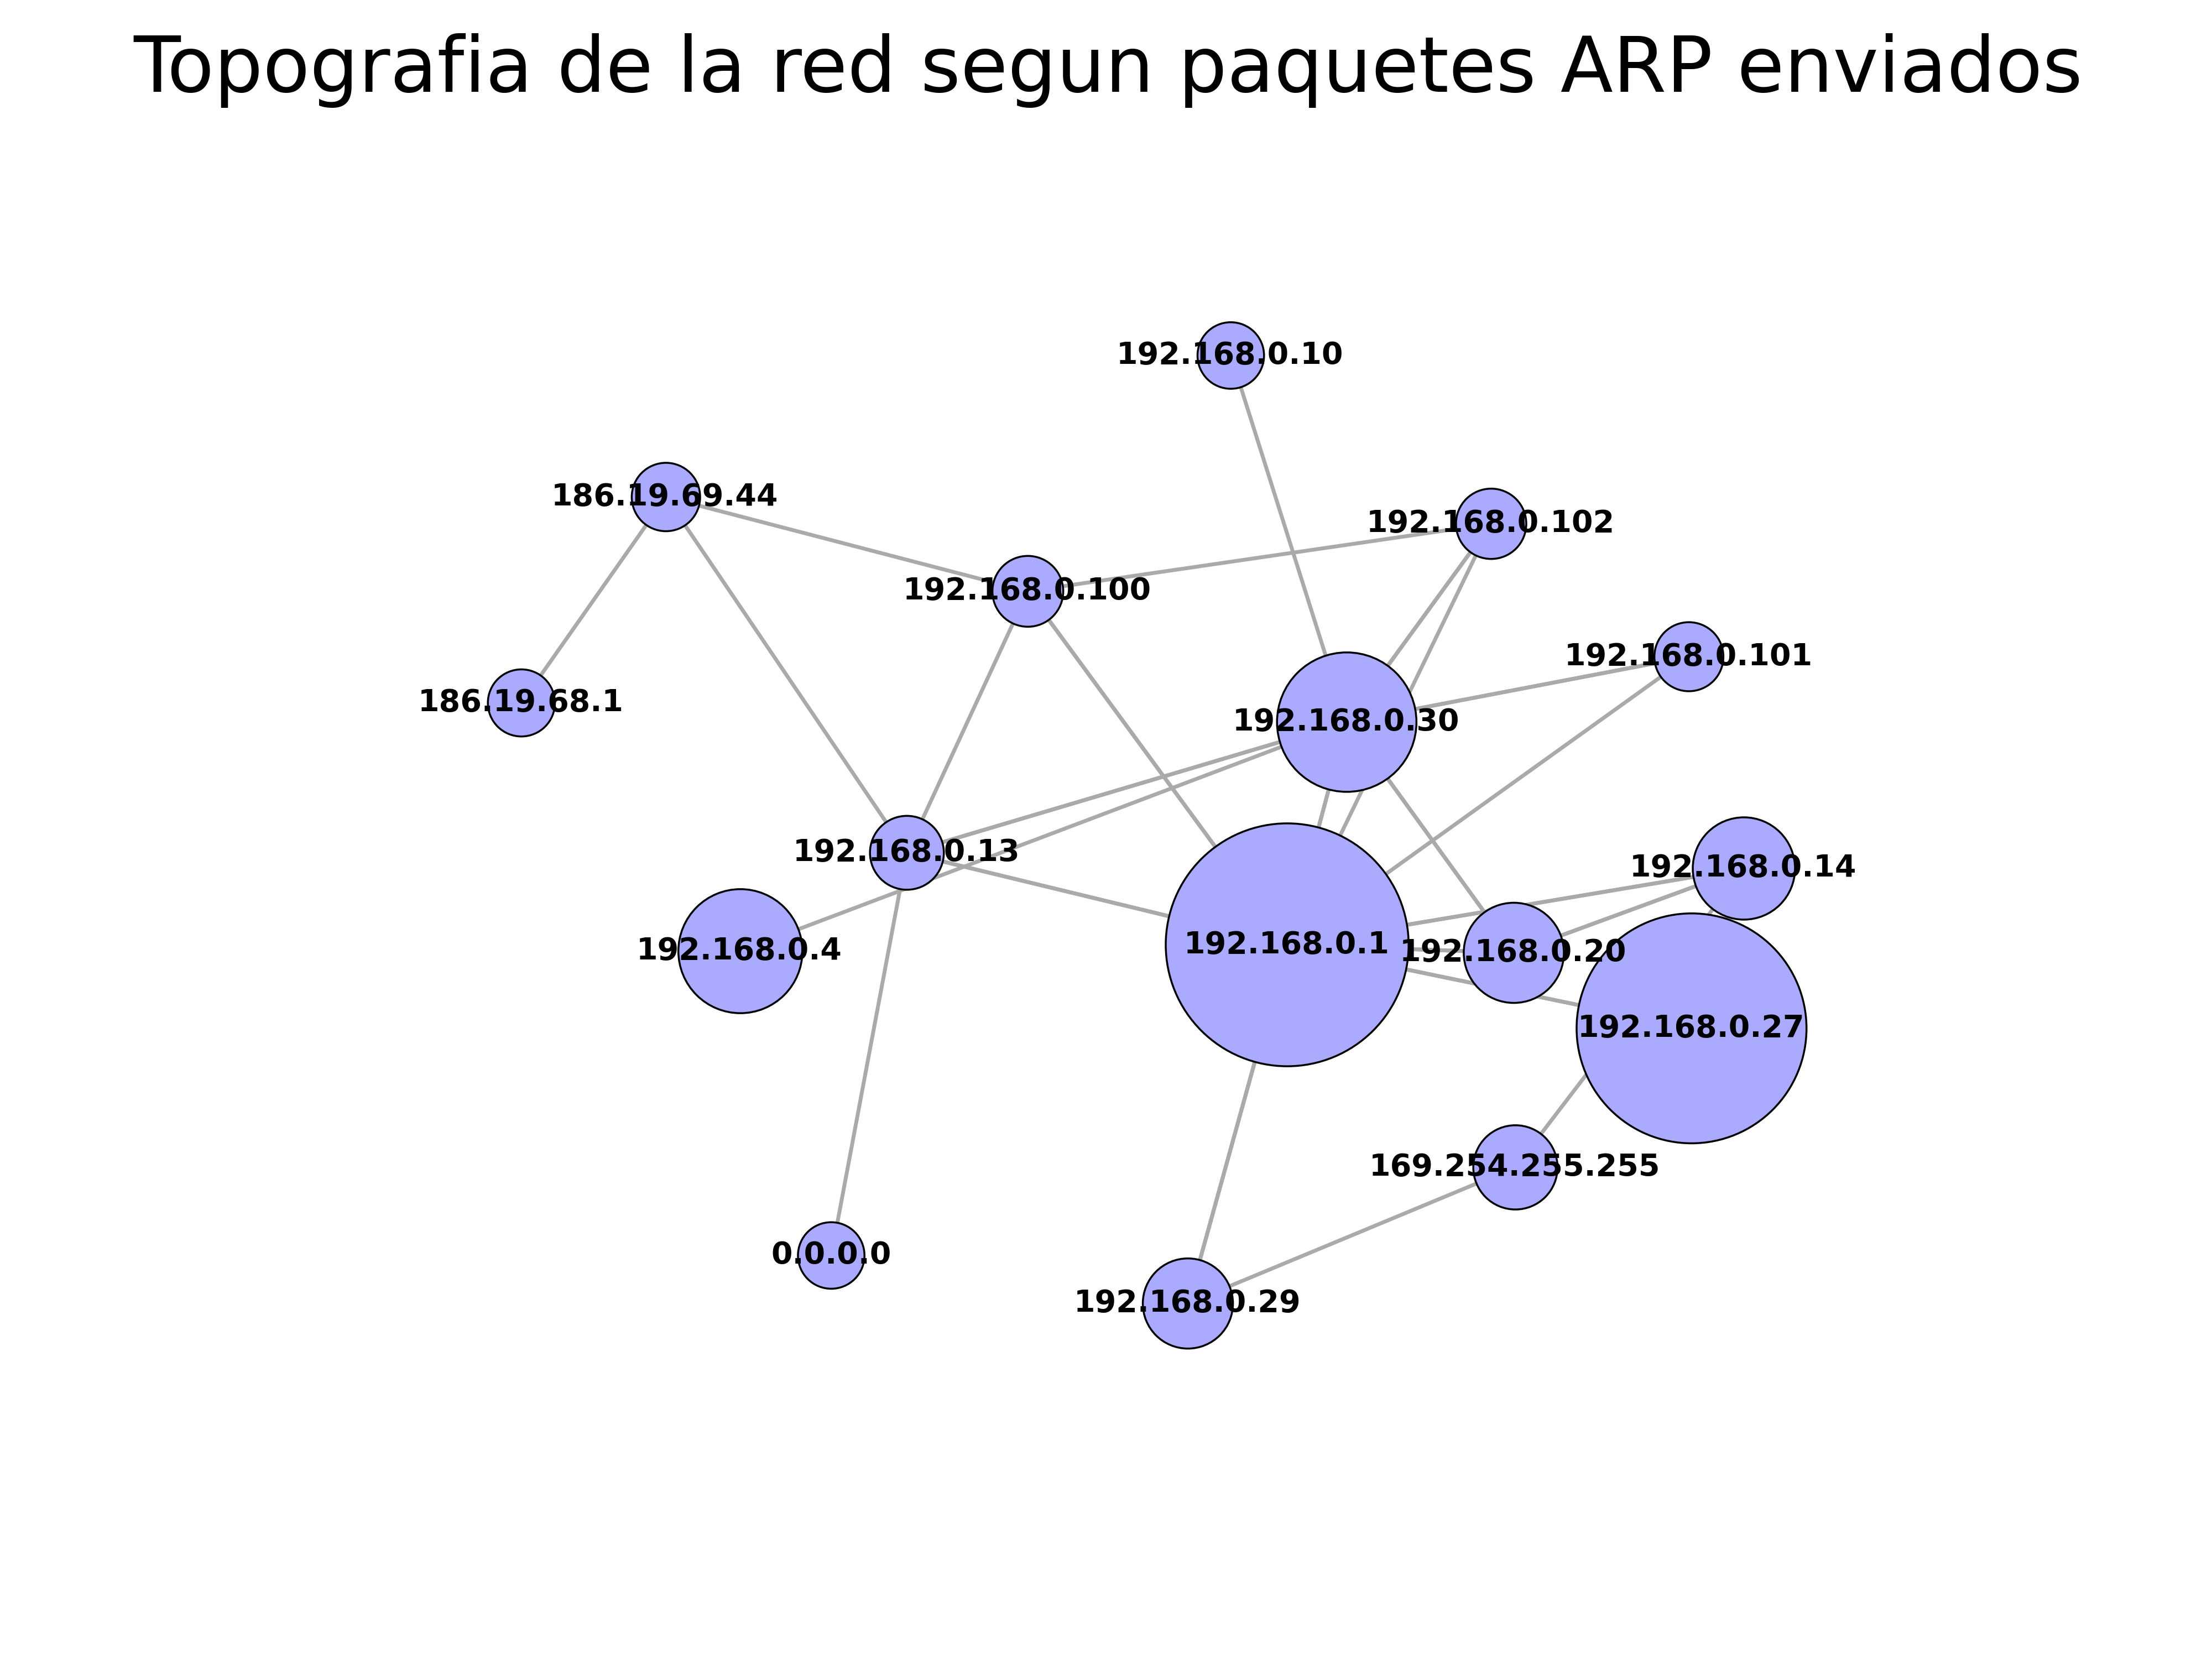
\includegraphics[width=0.7\textwidth]{graficos/red_domestica_network.png}
  \caption{Mi Figura}
  \label{fig:red_domestica_network}
\end{figure}

\FloatBarrier

\subsubsection{Histogramas (de IPs y protocolos)}

\begin{figure}[h!]
  \centering
   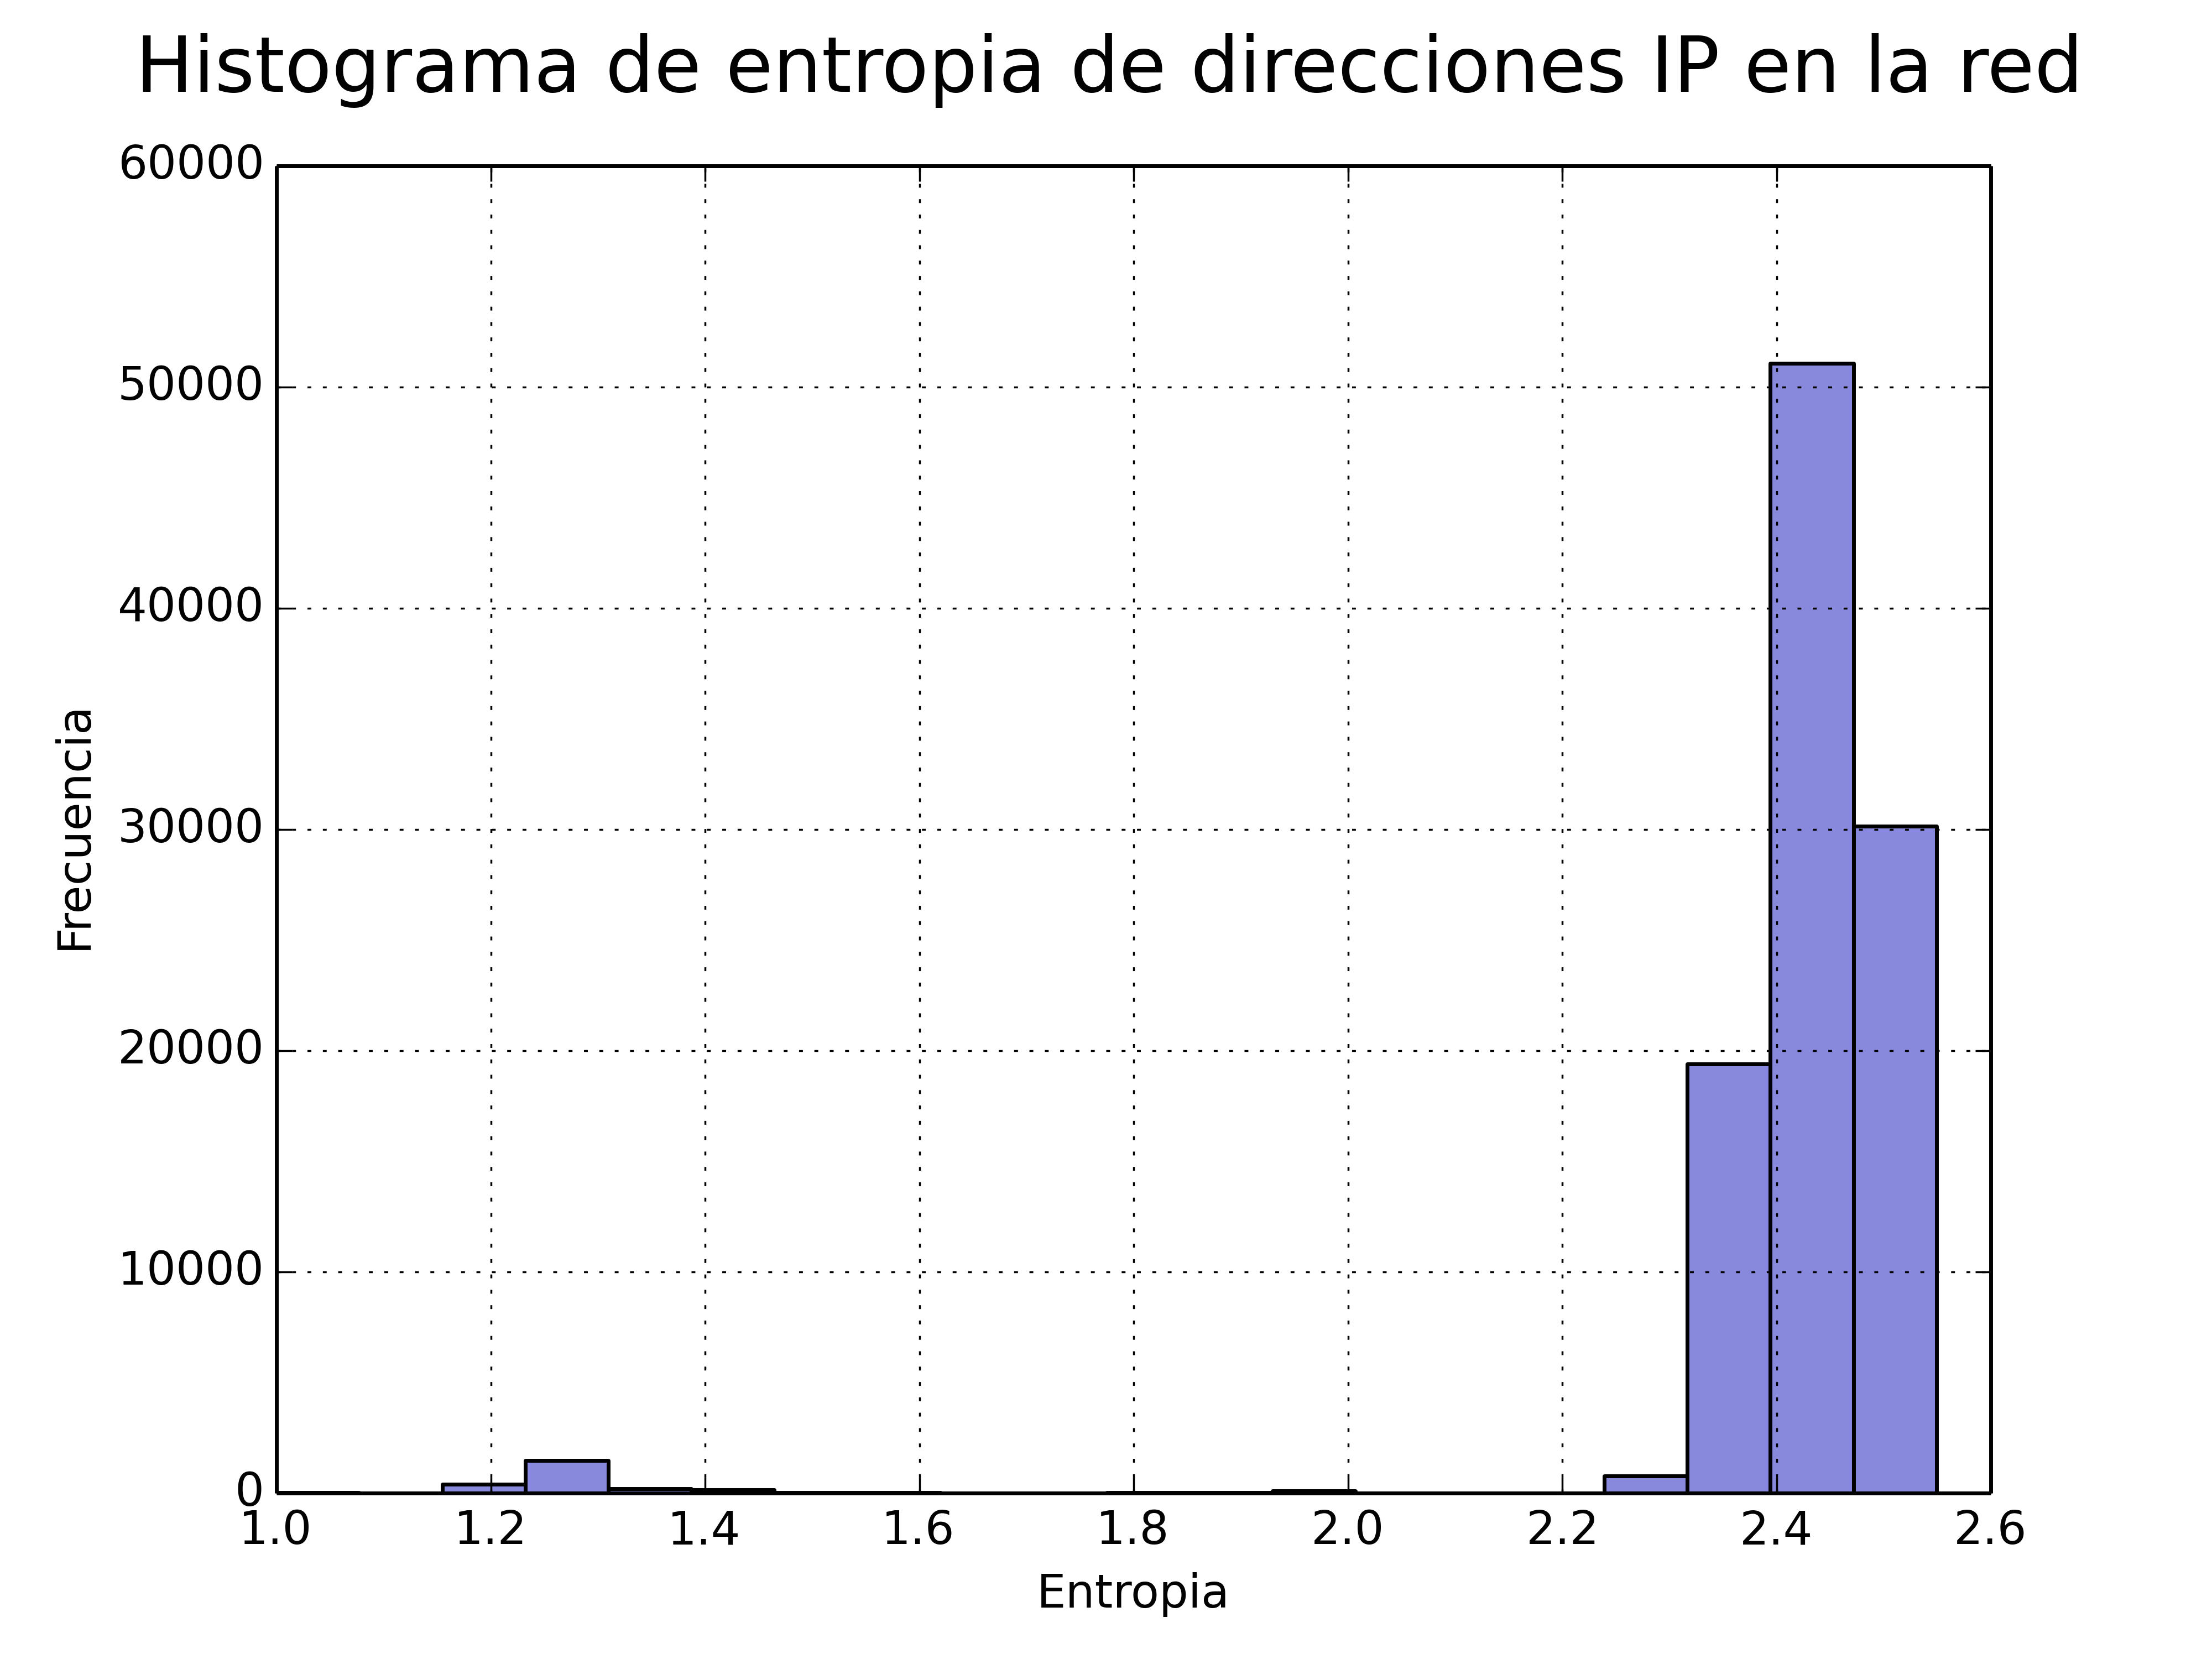
\includegraphics[width=0.7\textwidth]{graficos/red_domestica_hist_arp.png}
  \caption{Mi Figura}
  \label{fig:red_domestica_hist_arp}
\end{figure}

\begin{figure}[h!]
  \centering
   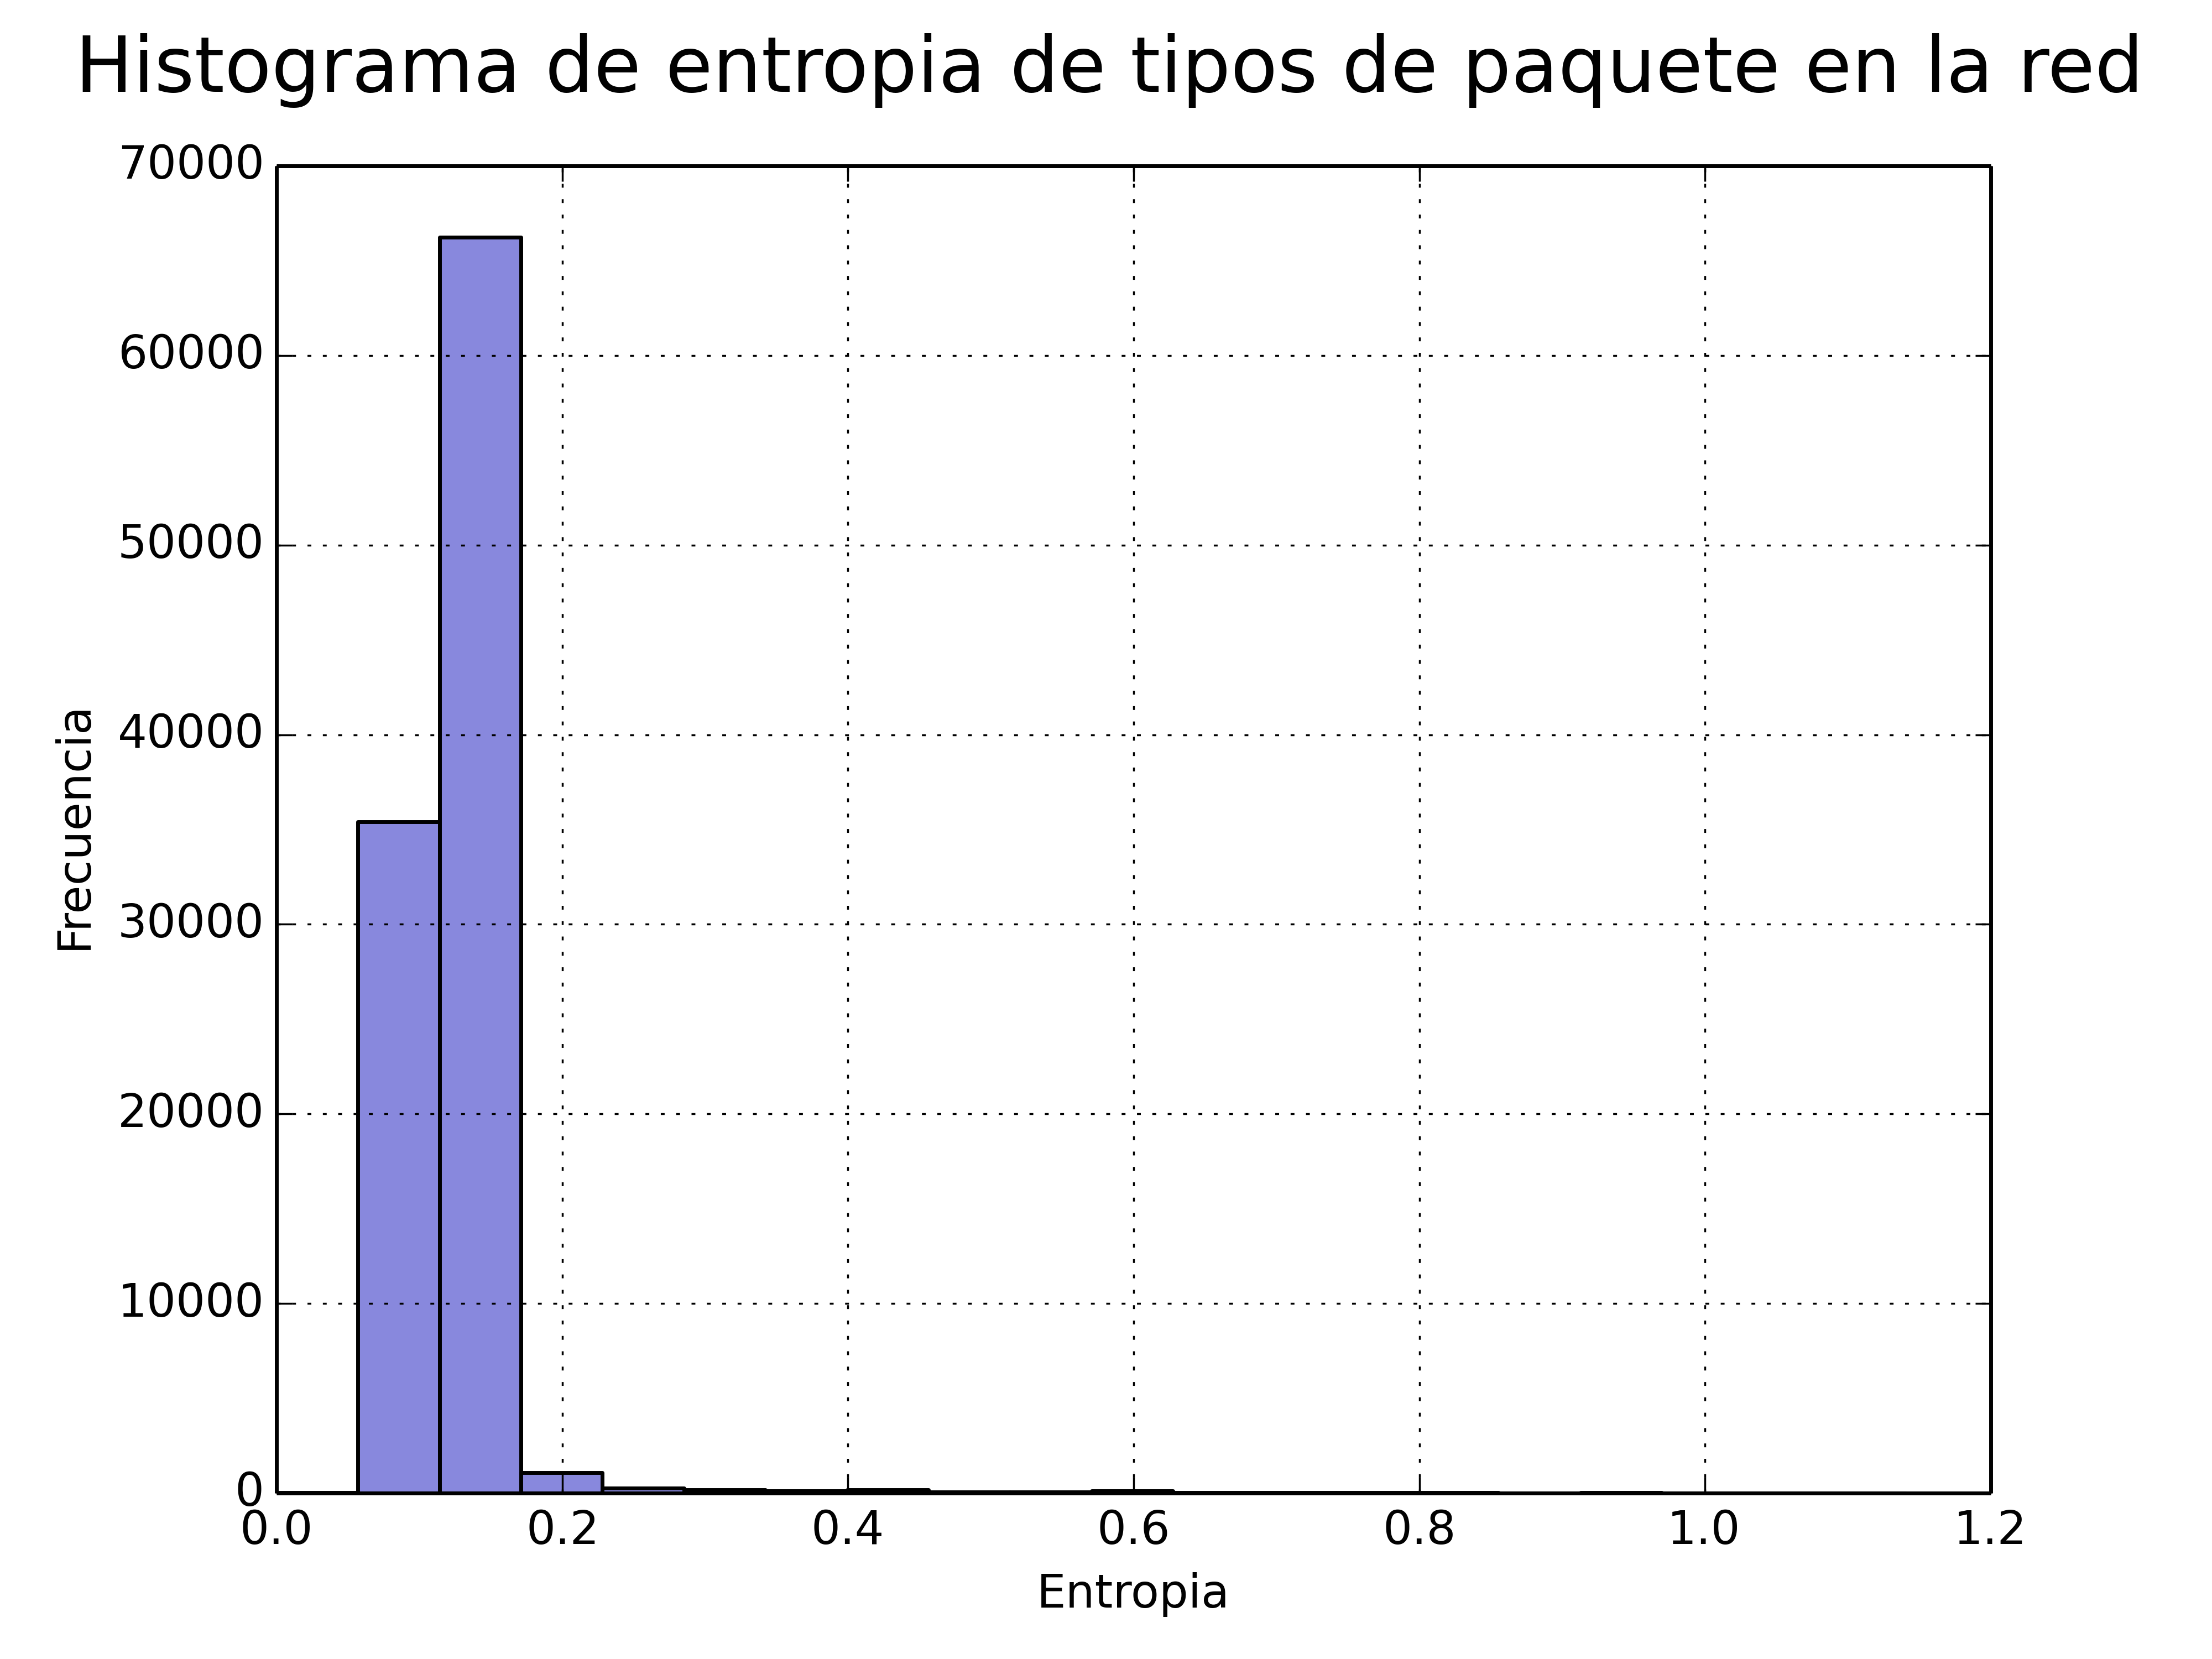
\includegraphics[width=0.7\textwidth]{graficos/red_domestica_hist_type.png}
  \caption{Mi Figura}
  \label{fig:red_domestica_hist_type}
\end{figure}

\FloatBarrier

\subsubsection{Paquetes capturados e información}

Los gráficos de torta, nos permiten ver la relación entre la cantidad de paquetes y la información que proveen cada nodo en la red. 
En los primeros 2 gráficos ~\ref{fig:red_domestica_pie_arp}. ~\ref{fig:red_domestica_pie_arp_information}. se toma como fuente las ips de la red.
Podemos notar que los nodos mencionados anteriormente son los mas frecuentes y por lo tanto los que menos información tienen.

En los siguientes 2 gráficos ~\ref{fig:red_domestica_pie_type}. ~\ref{fig:red_domestica_pie_type_information}. la fuente es la indicada en la cátedra. Vemos que el protocolo que mas se repite es el IP con un porcentaje muy superior al resto y aportando información casi nula. 

\begin{figure}[h!]
  \centering
   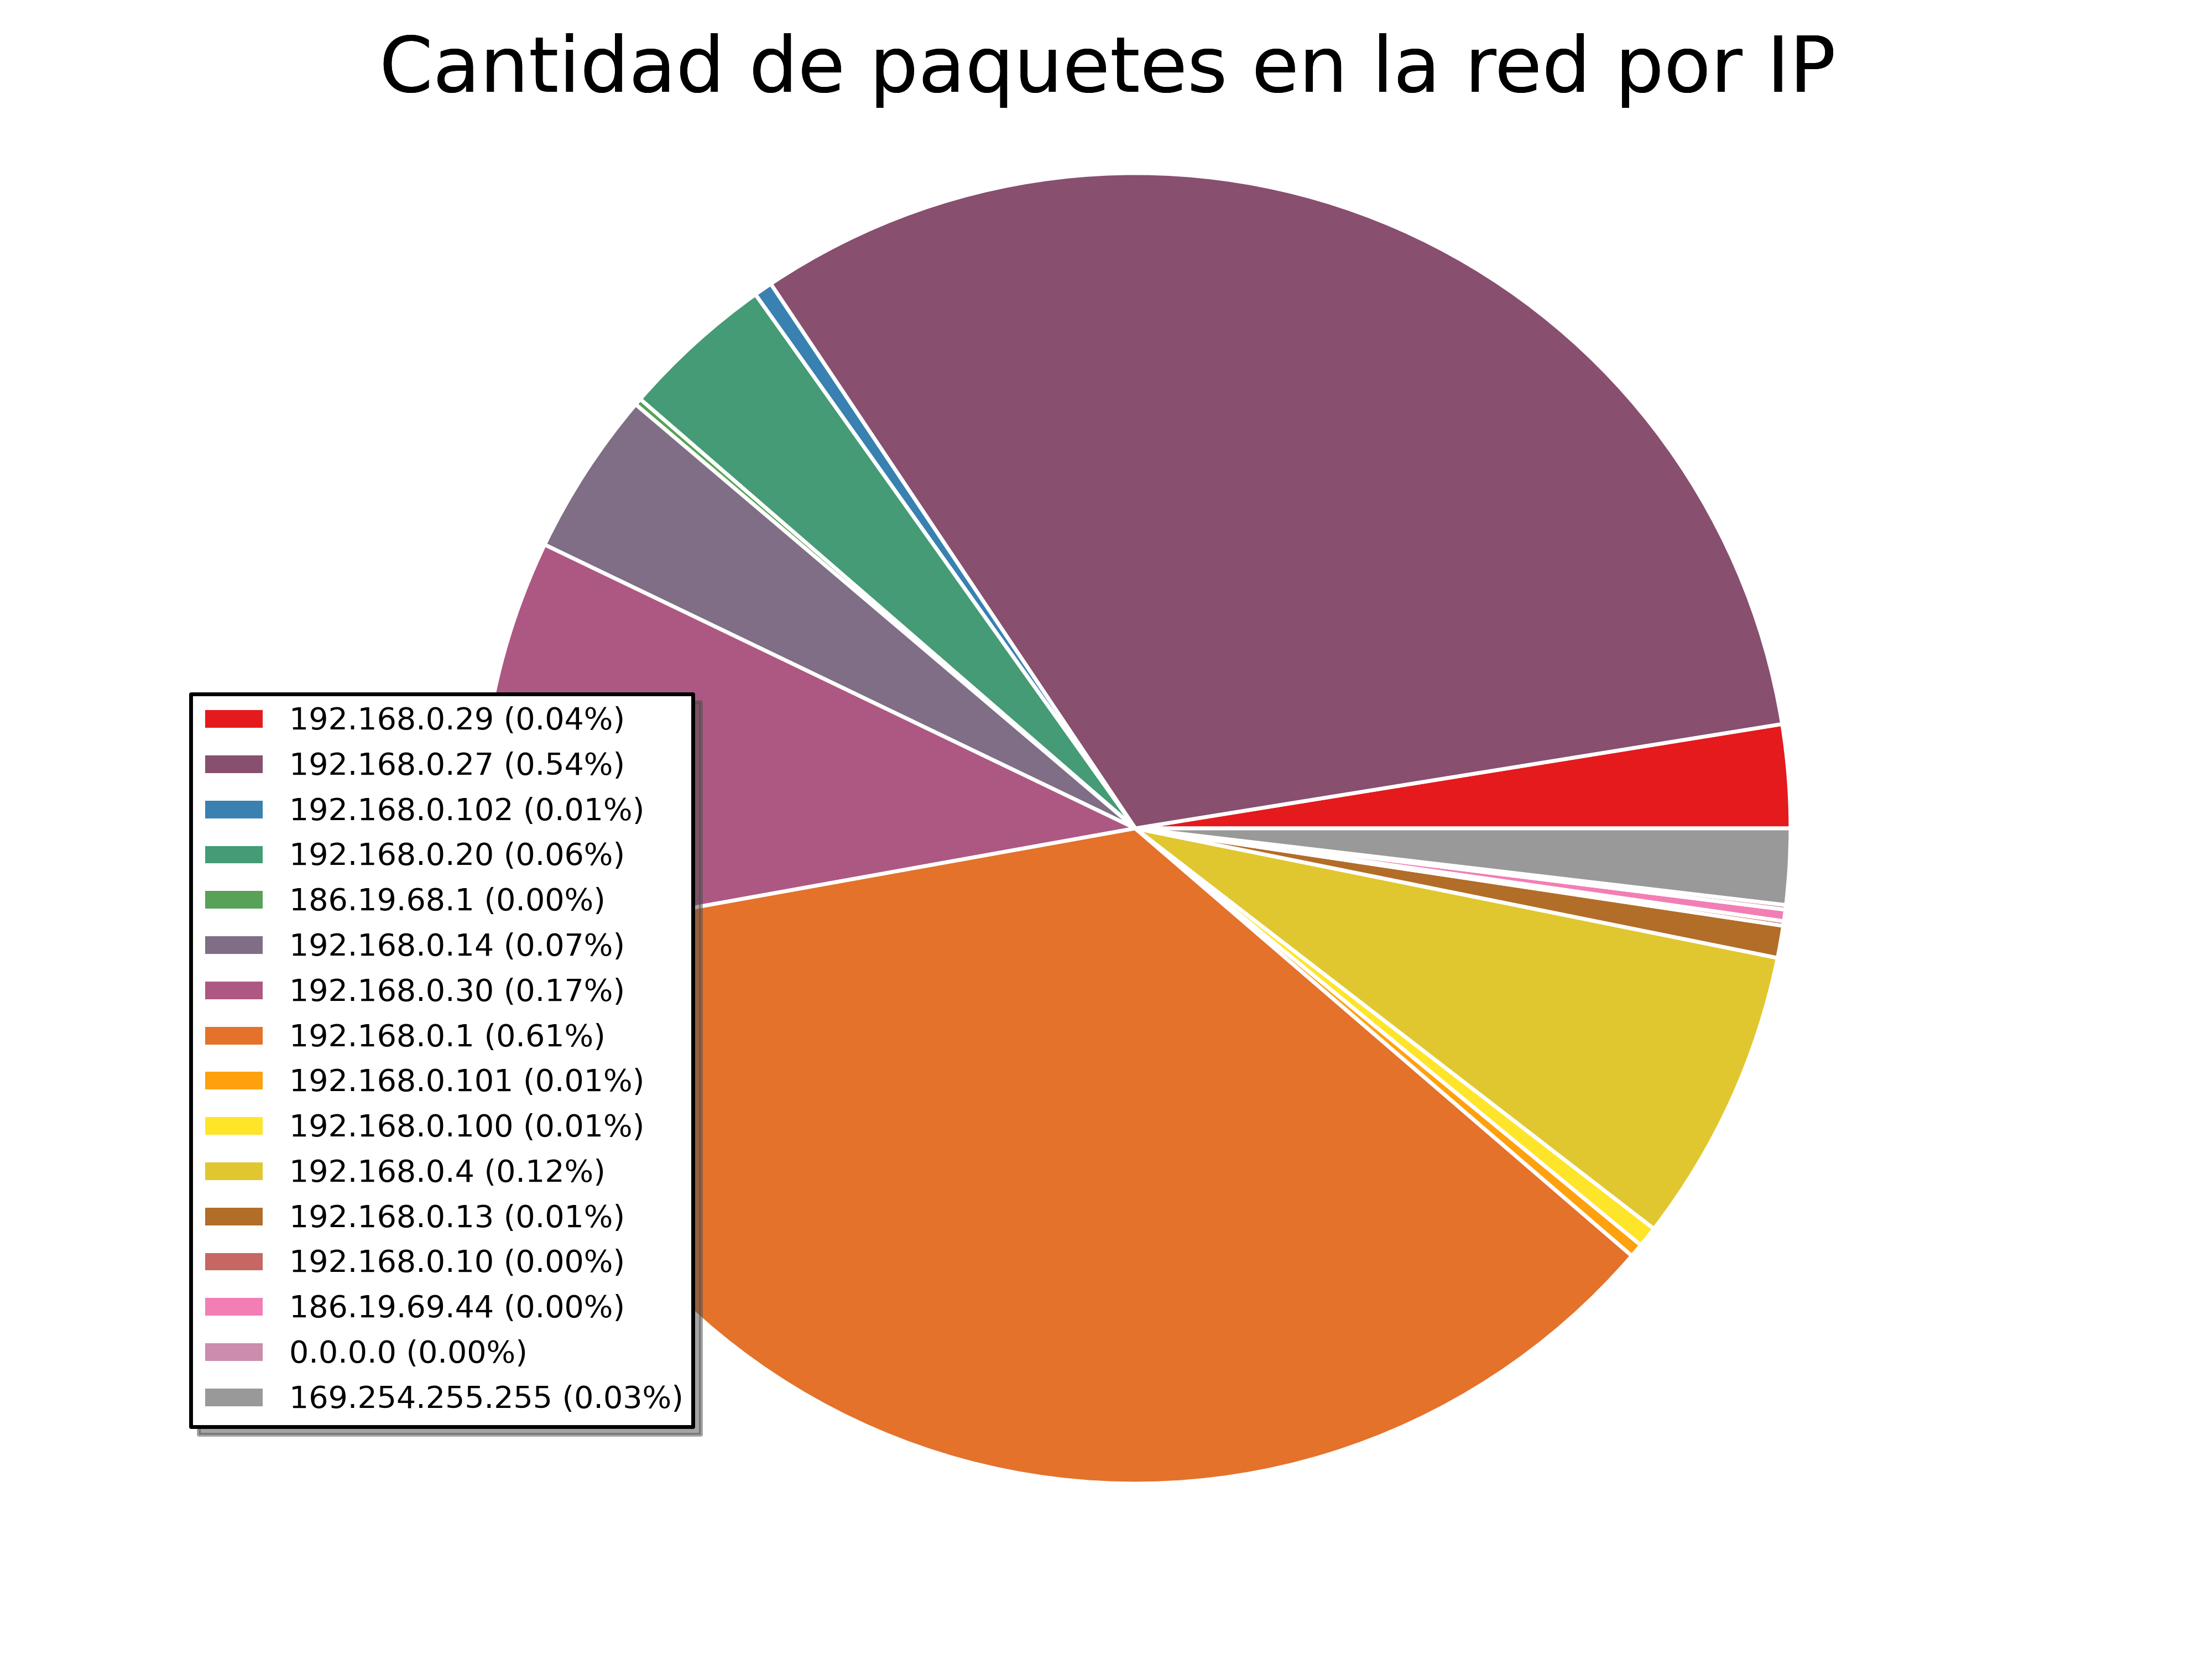
\includegraphics[width=0.7\textwidth]{graficos/red_domestica_pie_arp.png}
  \caption{Mi Figura}
  \label{fig:red_domestica_pie_arp}
\end{figure}

\begin{figure}[h!]
  \centering
   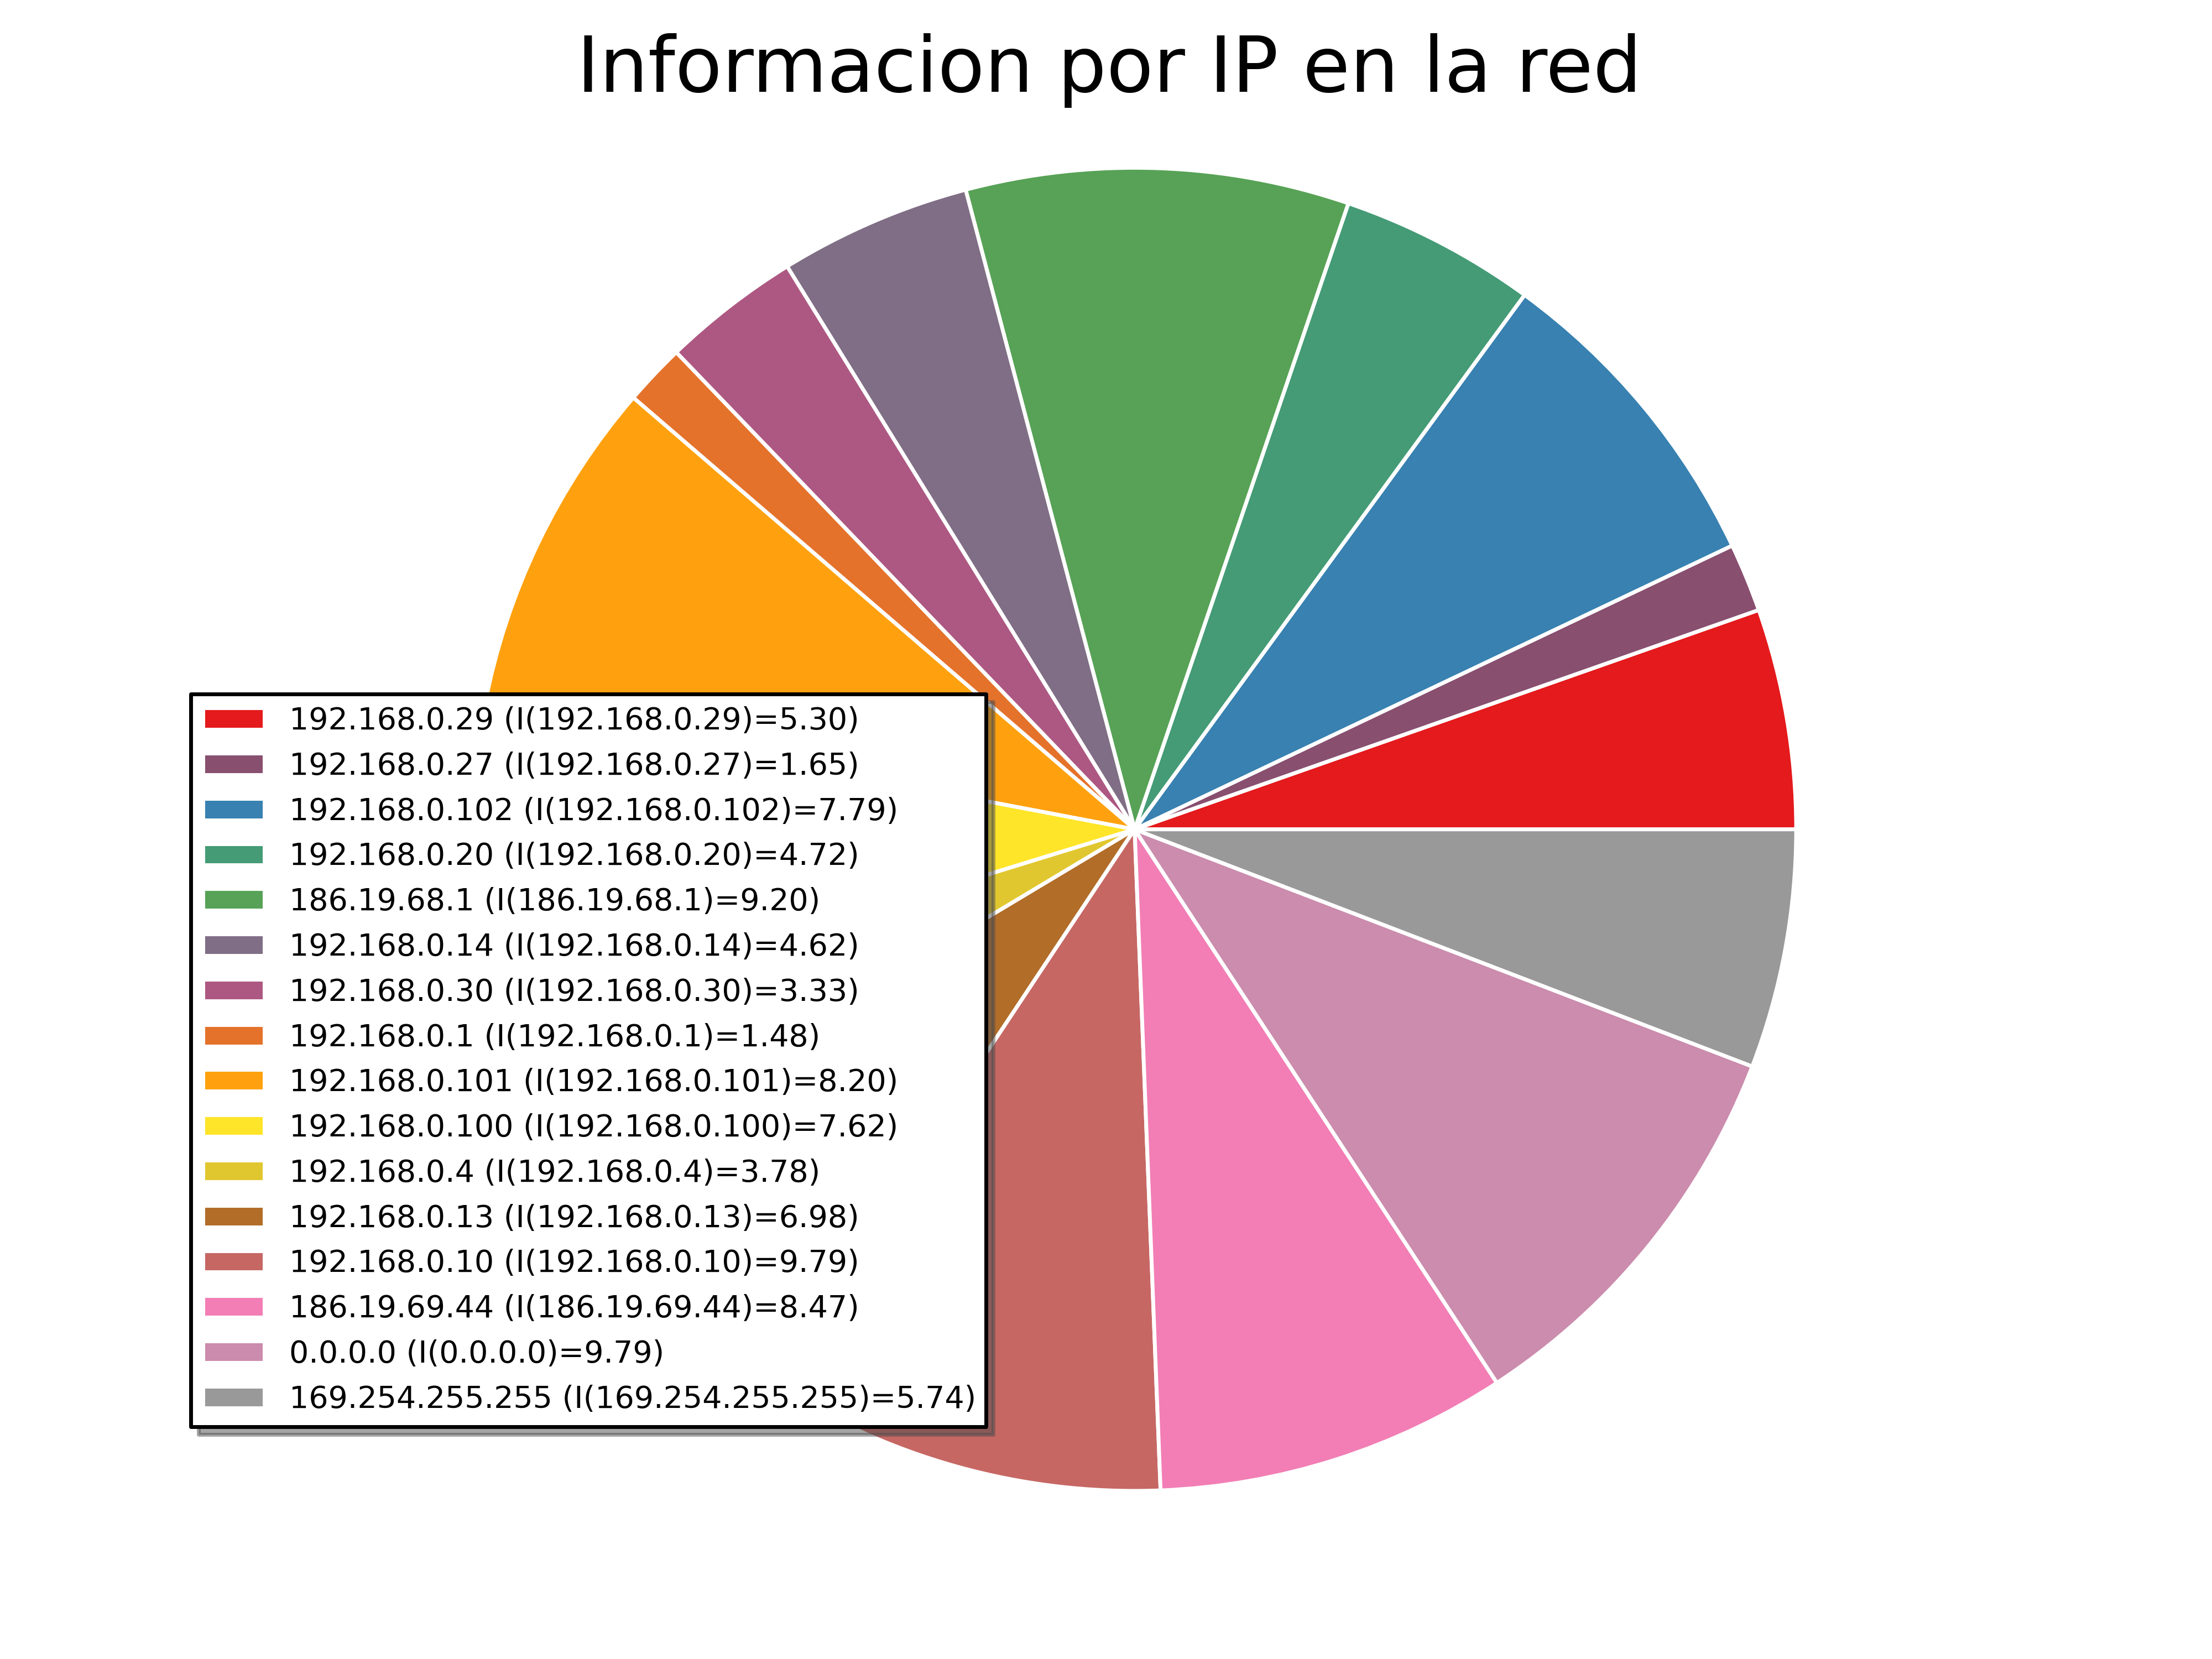
\includegraphics[width=0.7\textwidth]{graficos/red_domestica_pie_arp_information.png}
  \caption{Mi Figura}
  \label{fig:red_domestica_pie_arp_information}
\end{figure}

\begin{figure}[h!]
  \centering
   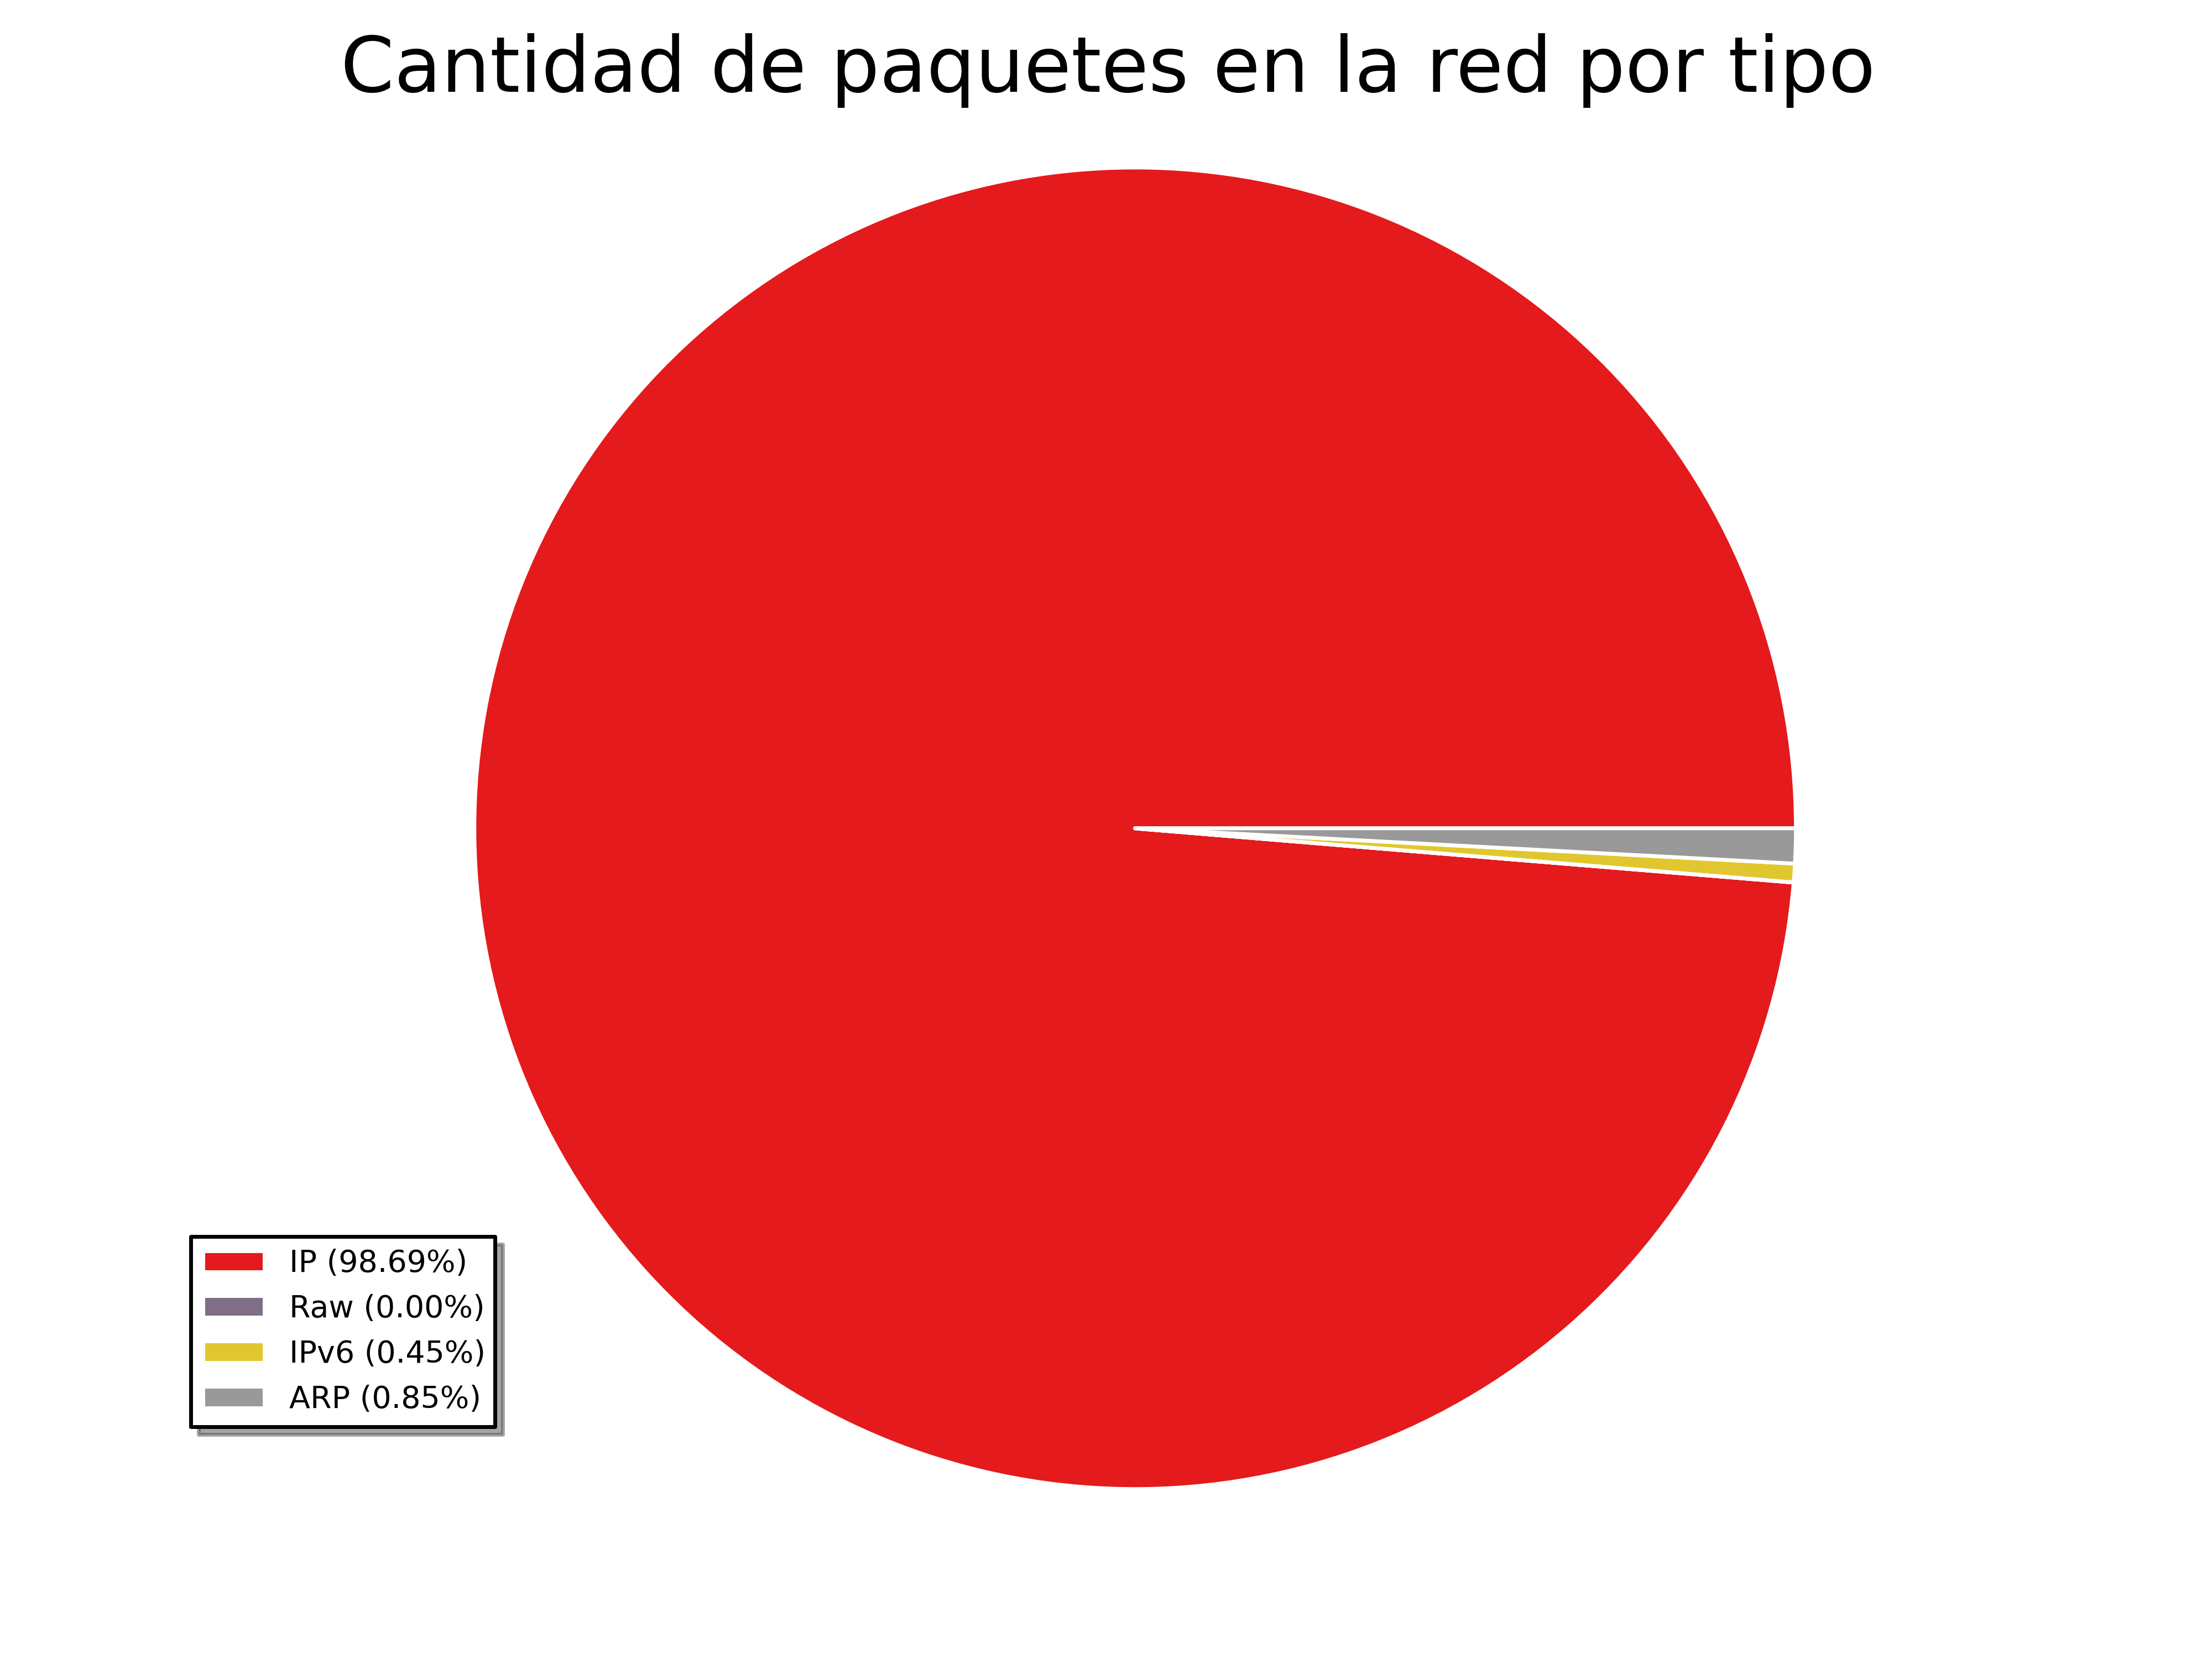
\includegraphics[width=0.7\textwidth]{graficos/red_domestica_pie_type.png}
  \caption{Mi Figura}
  \label{fig:red_domestica_pie_type}
\end{figure}

\begin{figure}[h!]
  \centering
   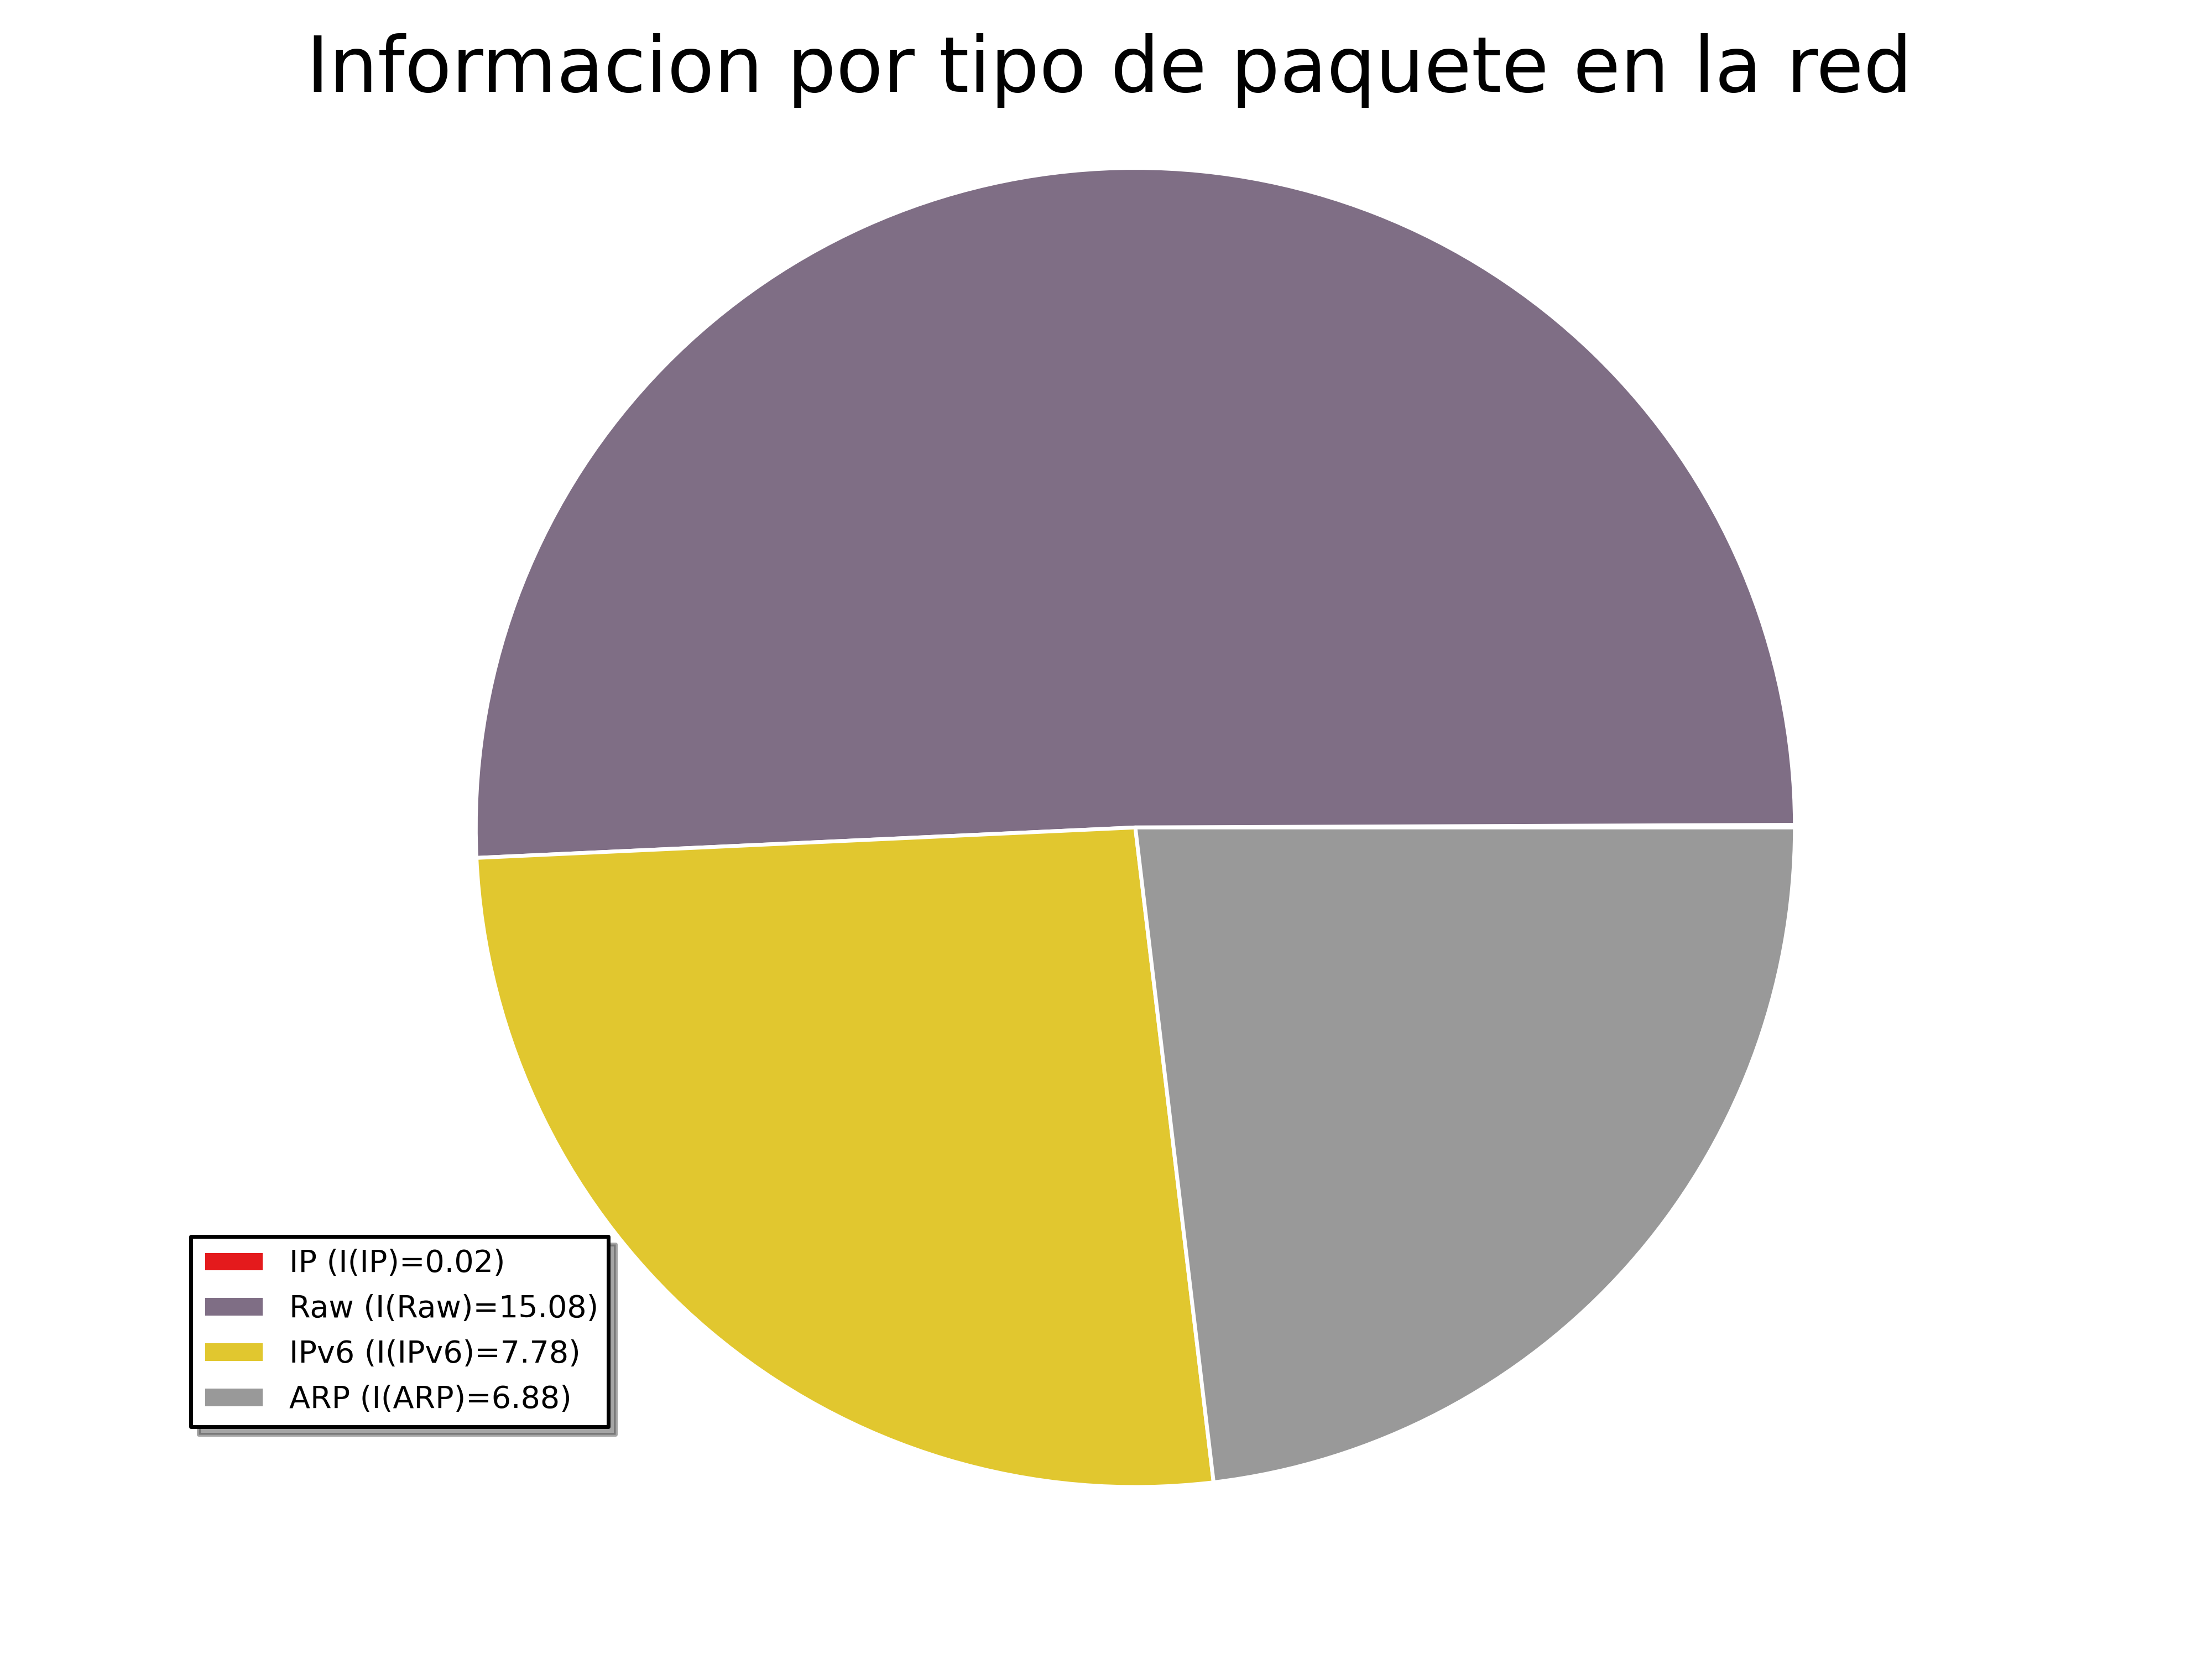
\includegraphics[width=0.7\textwidth]{graficos/red_domestica_pie_type_information.png}
  \caption{Mi Figura}
  \label{fig:red_domestica_pie_type_information}
\end{figure}
%\pagebreak
%\subsection{Red Laboral}

Esta captura se realizó en la red laboral de uno de los integrantes del grupo. Al ser una red con una gran cantidad de nodos y tráfico de paquetes, se optó por hacer las capturas al final de la jornada laboral donde el tráfico es menor. En otro momento los gráficos no resultaban claros para su análisis. La captura se realizó durante aproximadamente 10 minutos.
\\\\
Vemos a continuación el gráfico que muestra la topología de la red según el intercambio de paquetes ARP que hubo en la captura.

\FloatBarrier

\begin{figure}[ht!]
  \centering
   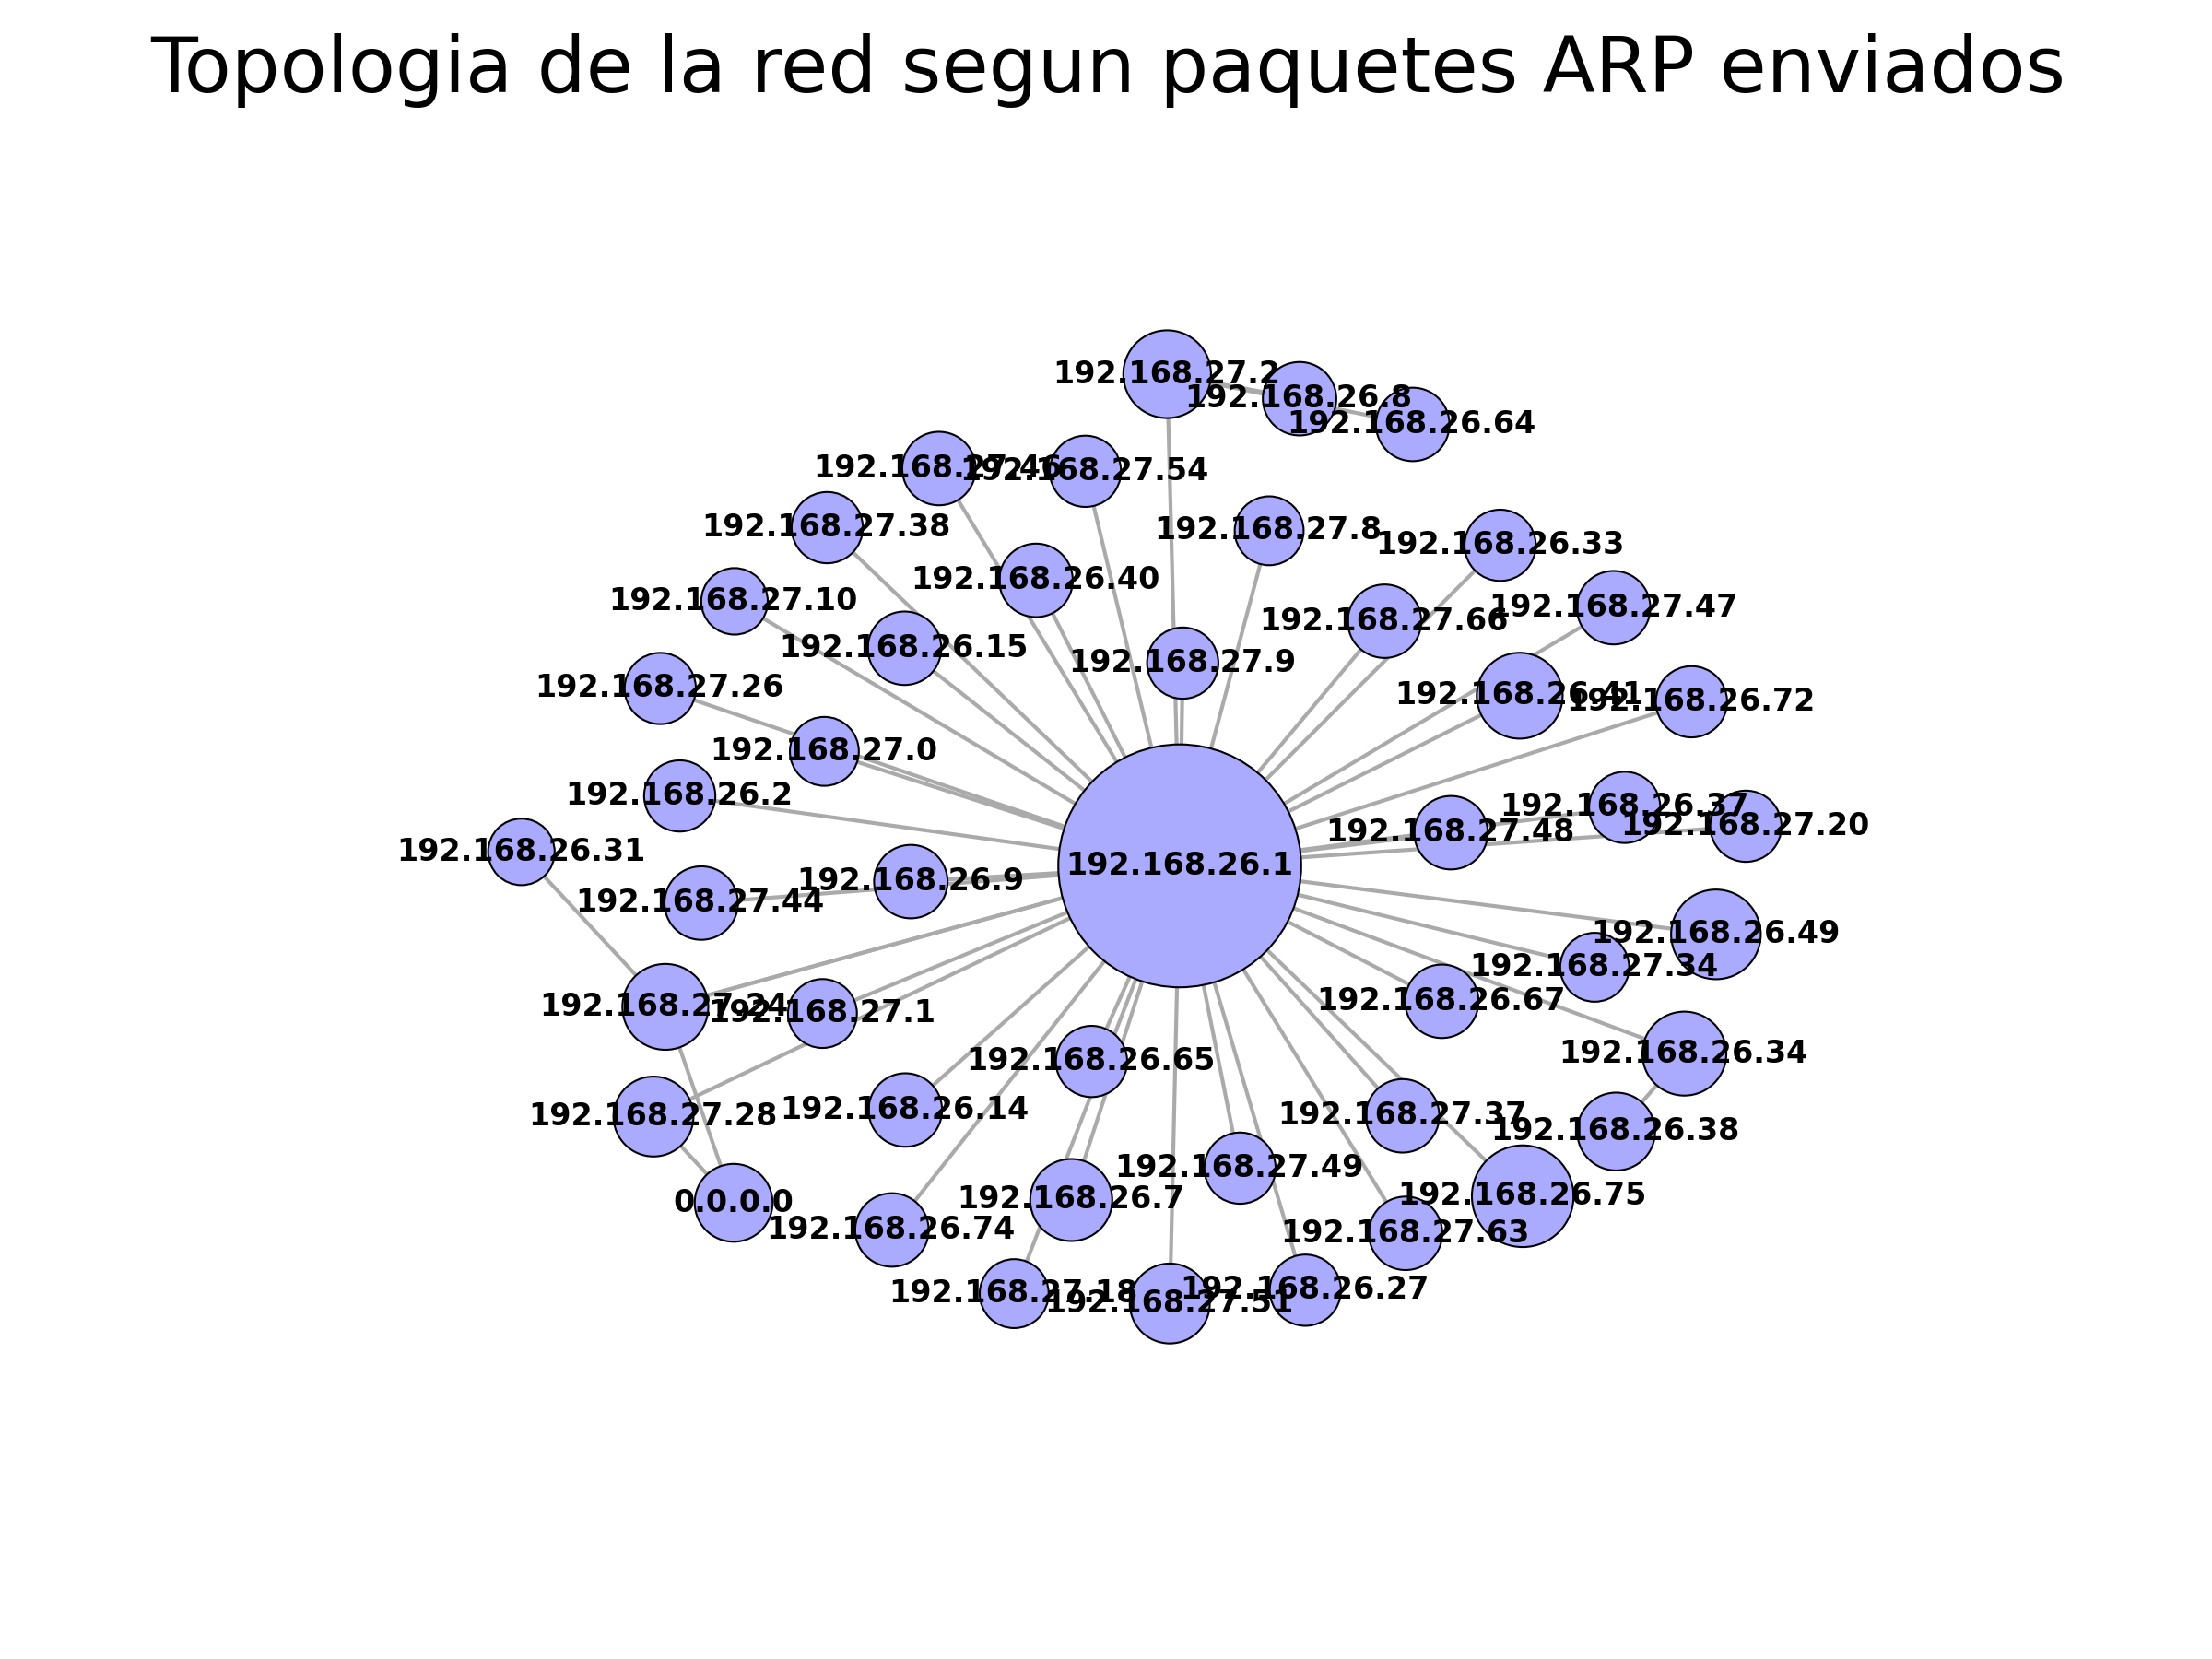
\includegraphics[width=0.7\textwidth]{graficos/laboral_network.png}
  \caption{}
  \label{fig:laboral_network}
\end{figure}

\FloatBarrier

En el centro del gráfico y de mayor tamaño podemos observar el nodo que representa al router con dirección IP 192.168.26.1. Por destacarse frente a los demás nodos creemos que este podría ser el nodo distinguido.
\\\\
Vemos ahora el gráfico que muestra la cantidad de información de cada nodo con respecto a la entropía.

\FloatBarrier

\begin{figure}[ht!]
  \centering
   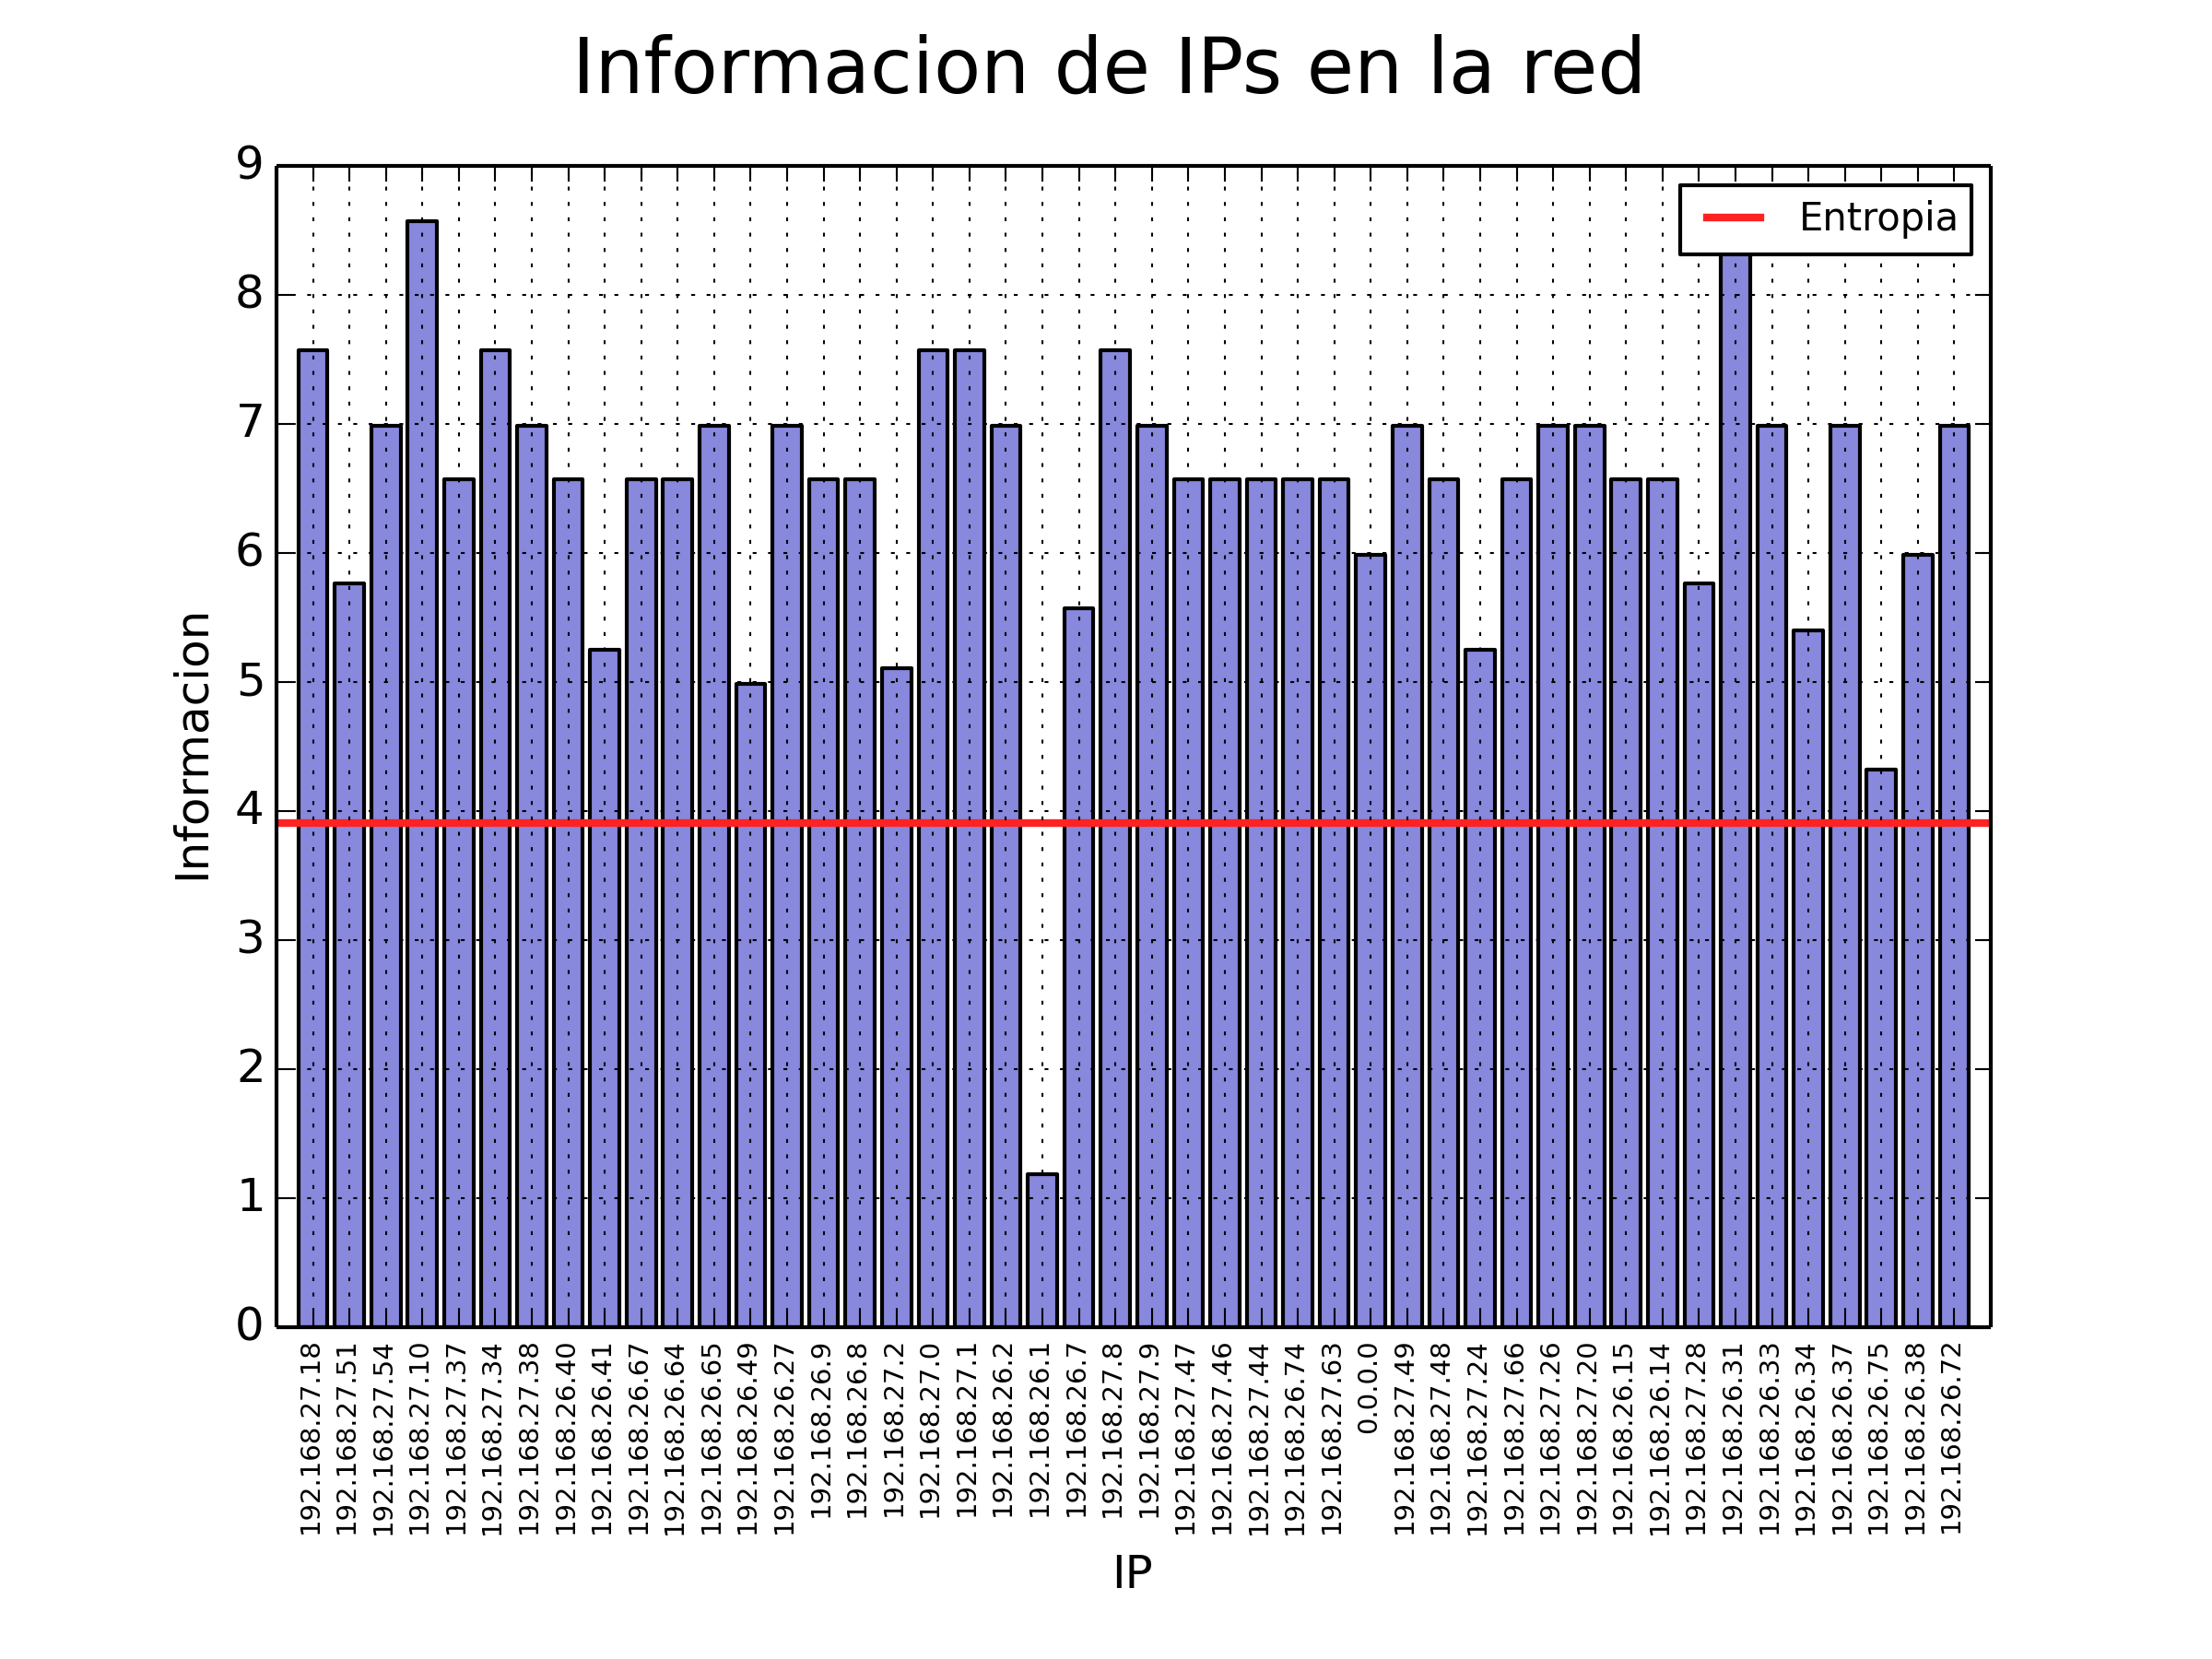
\includegraphics[width=0.7\textwidth]{graficos/laboral_information_bars_arp.png}
  \caption{}
  \label{fig:laboral_information_bars_arp}
\end{figure}

\FloatBarrier

Como podemos comprobar en este gráfico, la información que presenta el nodo correspondiente al router se encuentra muy por debajo de la entropía de la fuente. Por lo tanto concluímos que este es un nodo distinguido. Por otro lado vemos a un par de nodos que aportan mucha información, o sea que presentan una baja probabilidad. Posiblemente estos dos nodos sean equipos que tuvieron poca actividad durante la captura de paquetes, y participaron en pocas búsquedas ARP.
\\\\
Veremos a continuación el gráfico que muestra la cantidad de información de cada protocolo en comparación con la entropía.

\FloatBarrier

\begin{figure}[ht!]
  \centering
   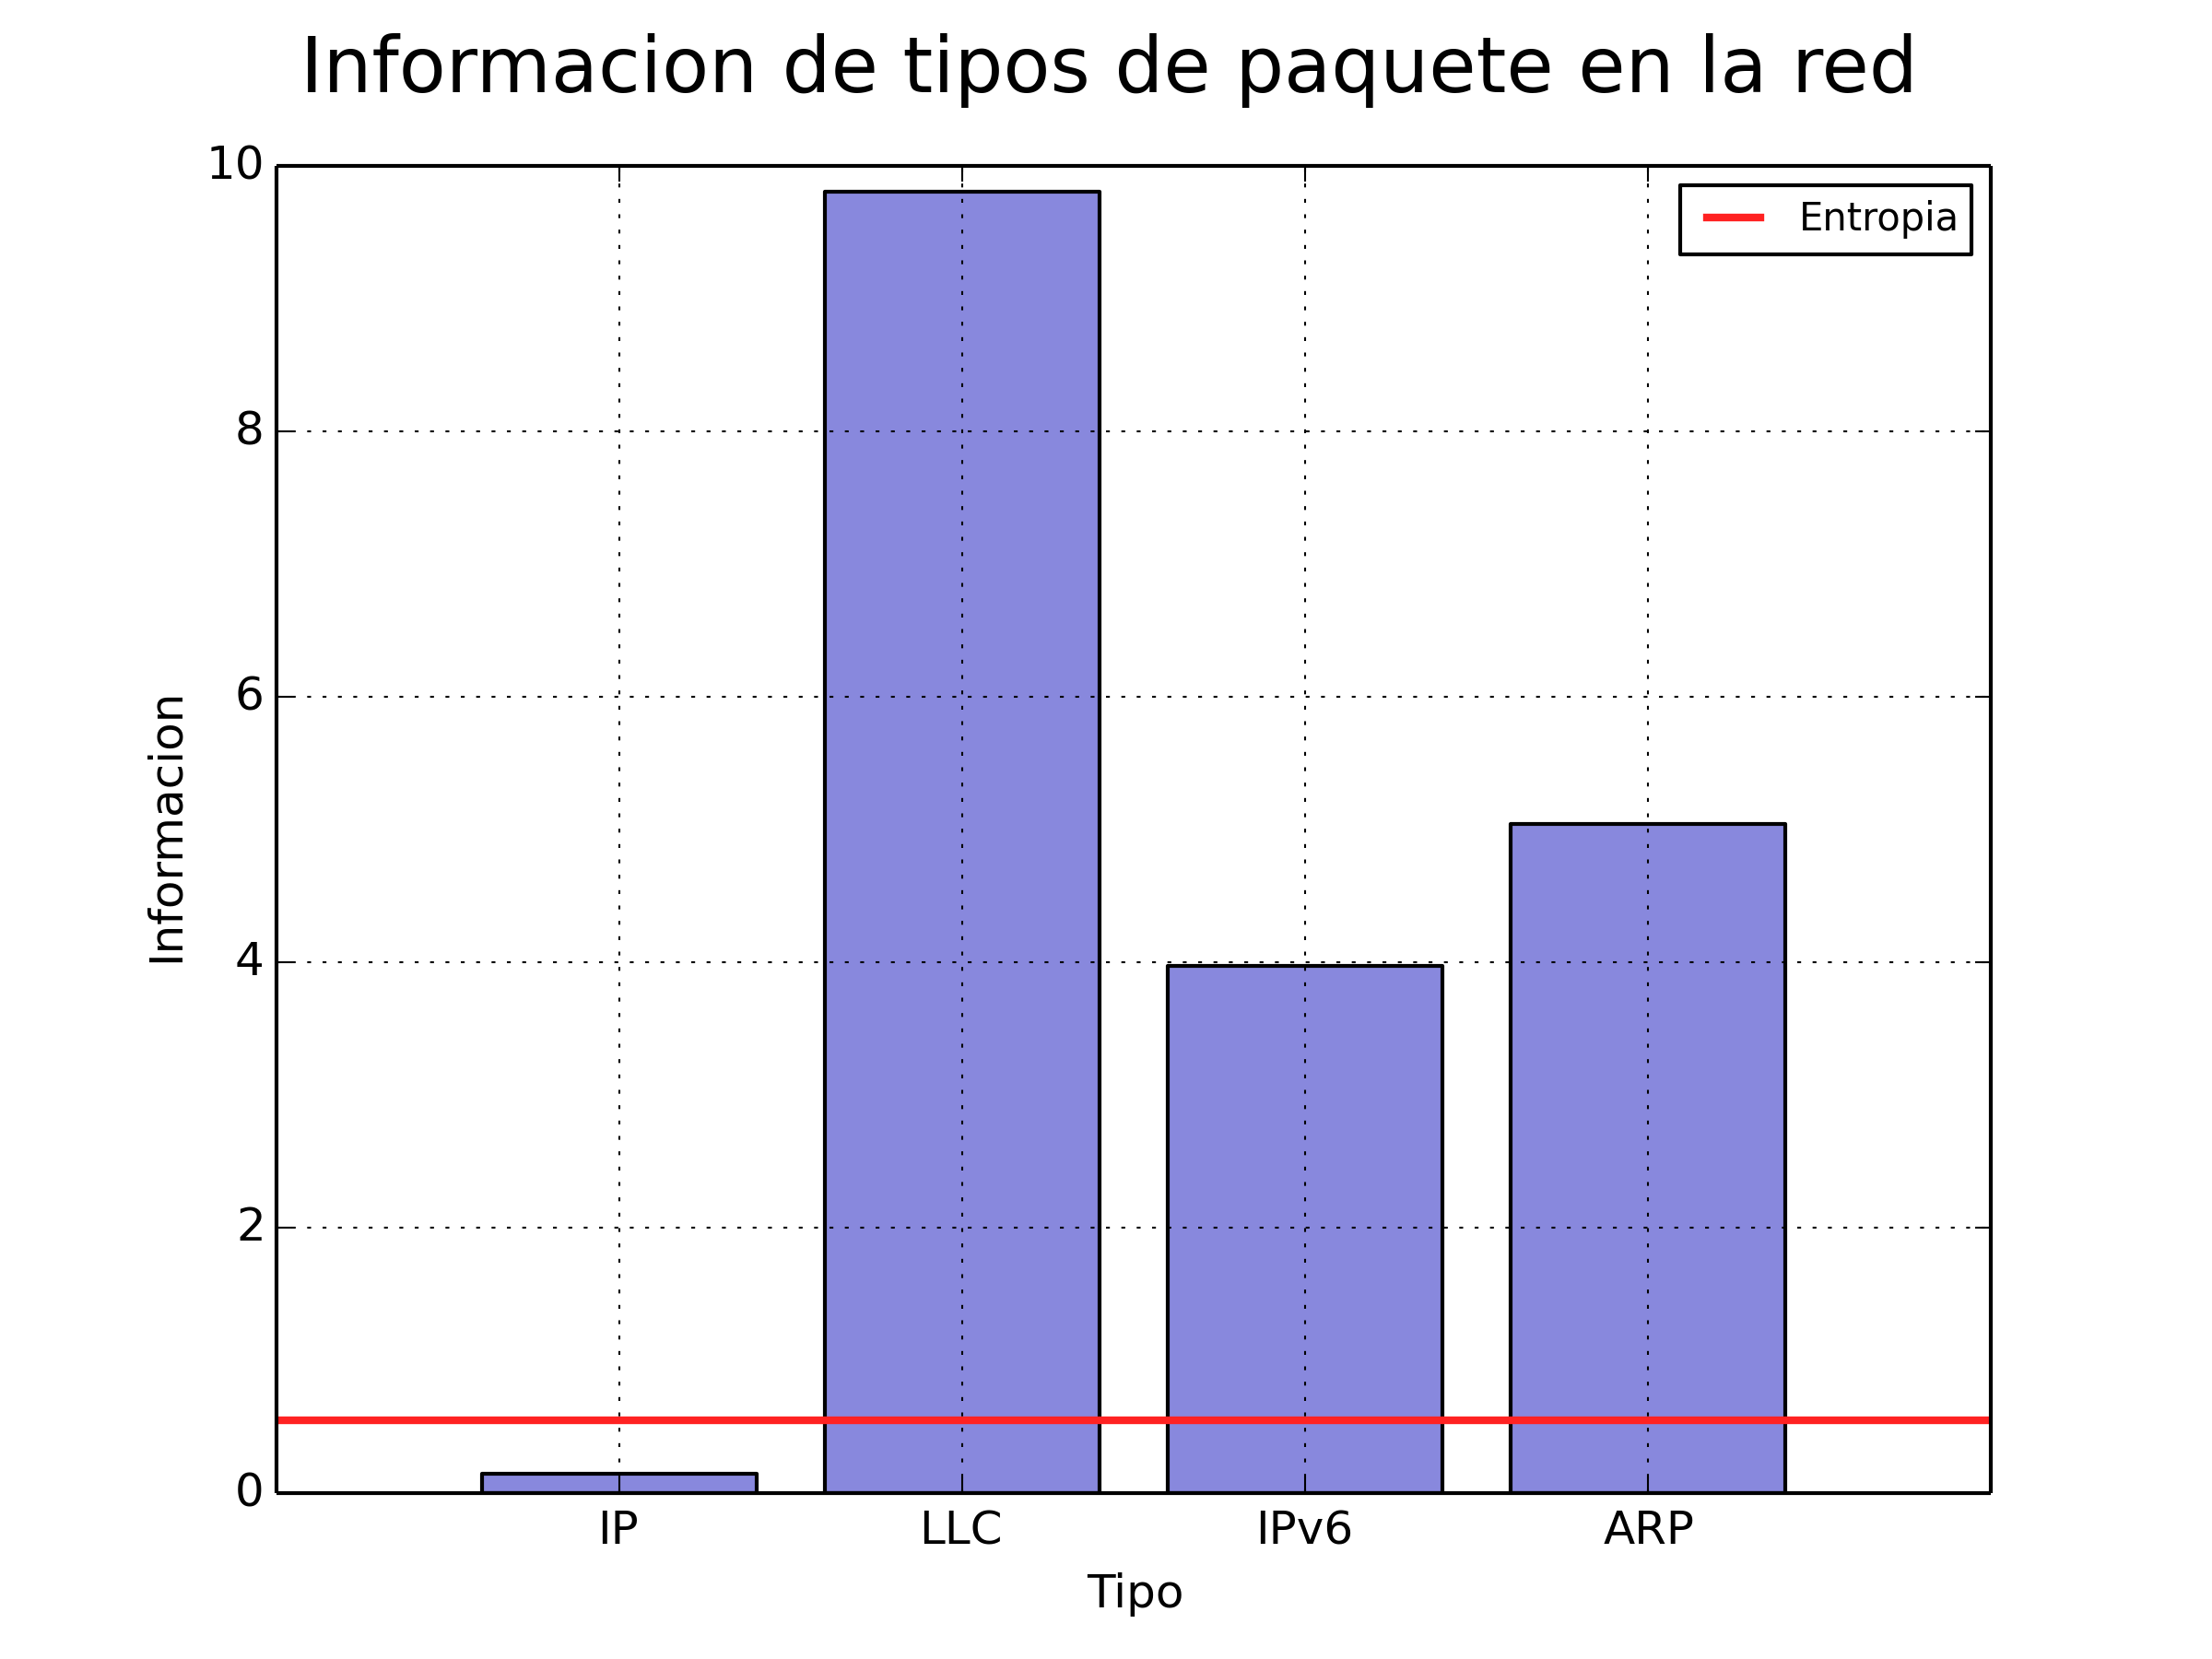
\includegraphics[width=0.7\textwidth]{graficos/laboral_information_bars_type.png}
  \caption{}
  \label{fig:laboral_information_bars_type}
\end{figure}

\FloatBarrier

Se pueden observar dos símbolos distinguidos. El protocolo IPv4, cuya información se presenta por debajo de la entropía. Es el protocolo que presenta más frecuencia y por este motivo aporta muy poca información.
Y el protocolo LLC que con muy poca frecuencia nos da mucha información.
También podemos observar que la cantidad de paquetes ARP e IPv6, en comparación con la de IPv4, es baja.
%\pagebreak
%\subsection{Red de Centro Comercial}

En este caso la captura se llevó a cabo en una red no controlada, en el shopping Galerías Pacífico, durante aproximadamente 10 minutos.
Debido a que la red no está controlada por nosotros, no conocemos detalles de la naturaleza de los equipos que intercambian información en la misma. Pero conjeturamos que la mayoría podrían ser teléfonos celulares.
\\\\
Vemos a continuación el gráfico que muestra la topología según la captura.

\FloatBarrier

\begin{figure}[ht!]
  \centering
   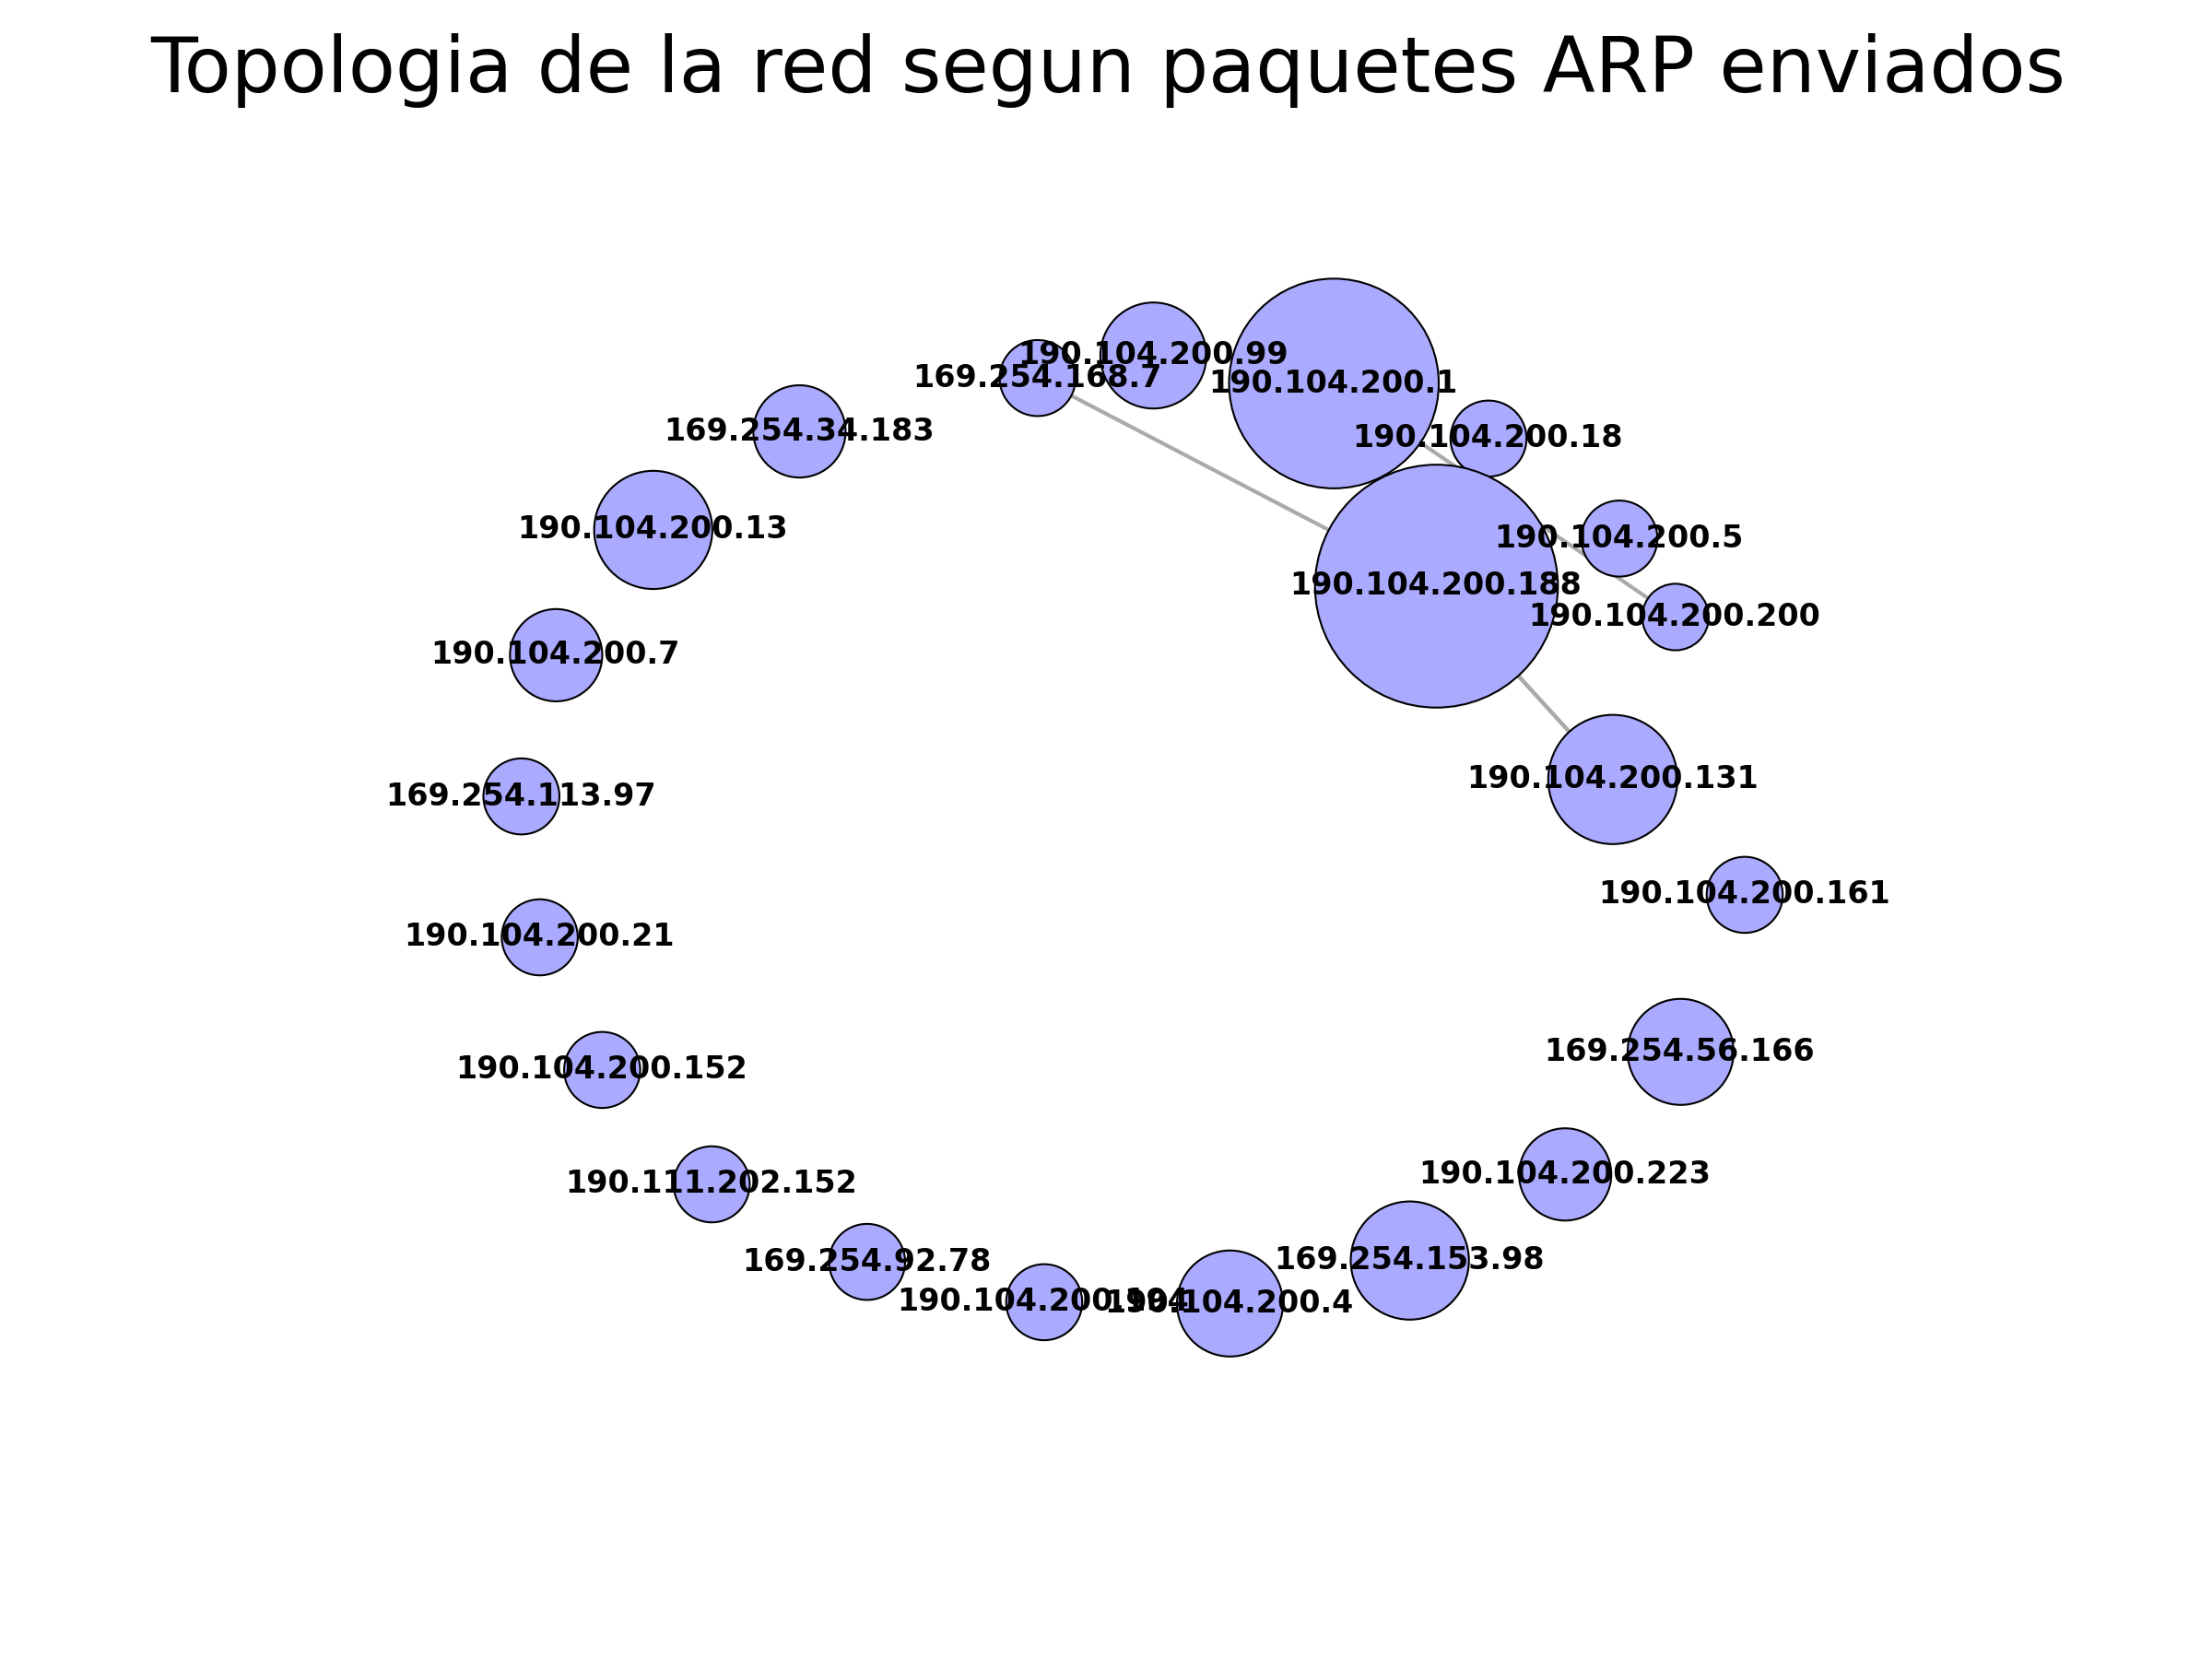
\includegraphics[width=0.7\textwidth]{graficos/shopping_network.png}
  \caption{}
  \label{fig:shopping_network}
\end{figure}

\FloatBarrier

En este diagrama podemos observar que la mayoría de los nodos se encuentran sin un eje que los conecte. Esto se debe a que durante la captura, en general los paquetes ARP tuvieron la misma dirección IP como origen y destino. Según lo que investigamos sobre este comportamiento se debe a una práctica llamada ARP gratuitos. Los paquetes ARP gratuitos contienen en el destino la misma dirección IP que la del origen quien lo envía y la MAC destino es una dirección broadcast. La utilidad de este tipo de paquetes es la de poder detectar conflictos de direcciones IP duplicadas. También se utilizan para informar a los switches, o máquinas,de las MAC de sus interfaces para que actualicen sus tablas sin necesidad de peticiones directas.
\\\\
Observamos a continuación el gráfico de cantidad de información de cada nodo con respecto a la entropía.

\FloatBarrier

\begin{figure}[ht!]
  \centering
   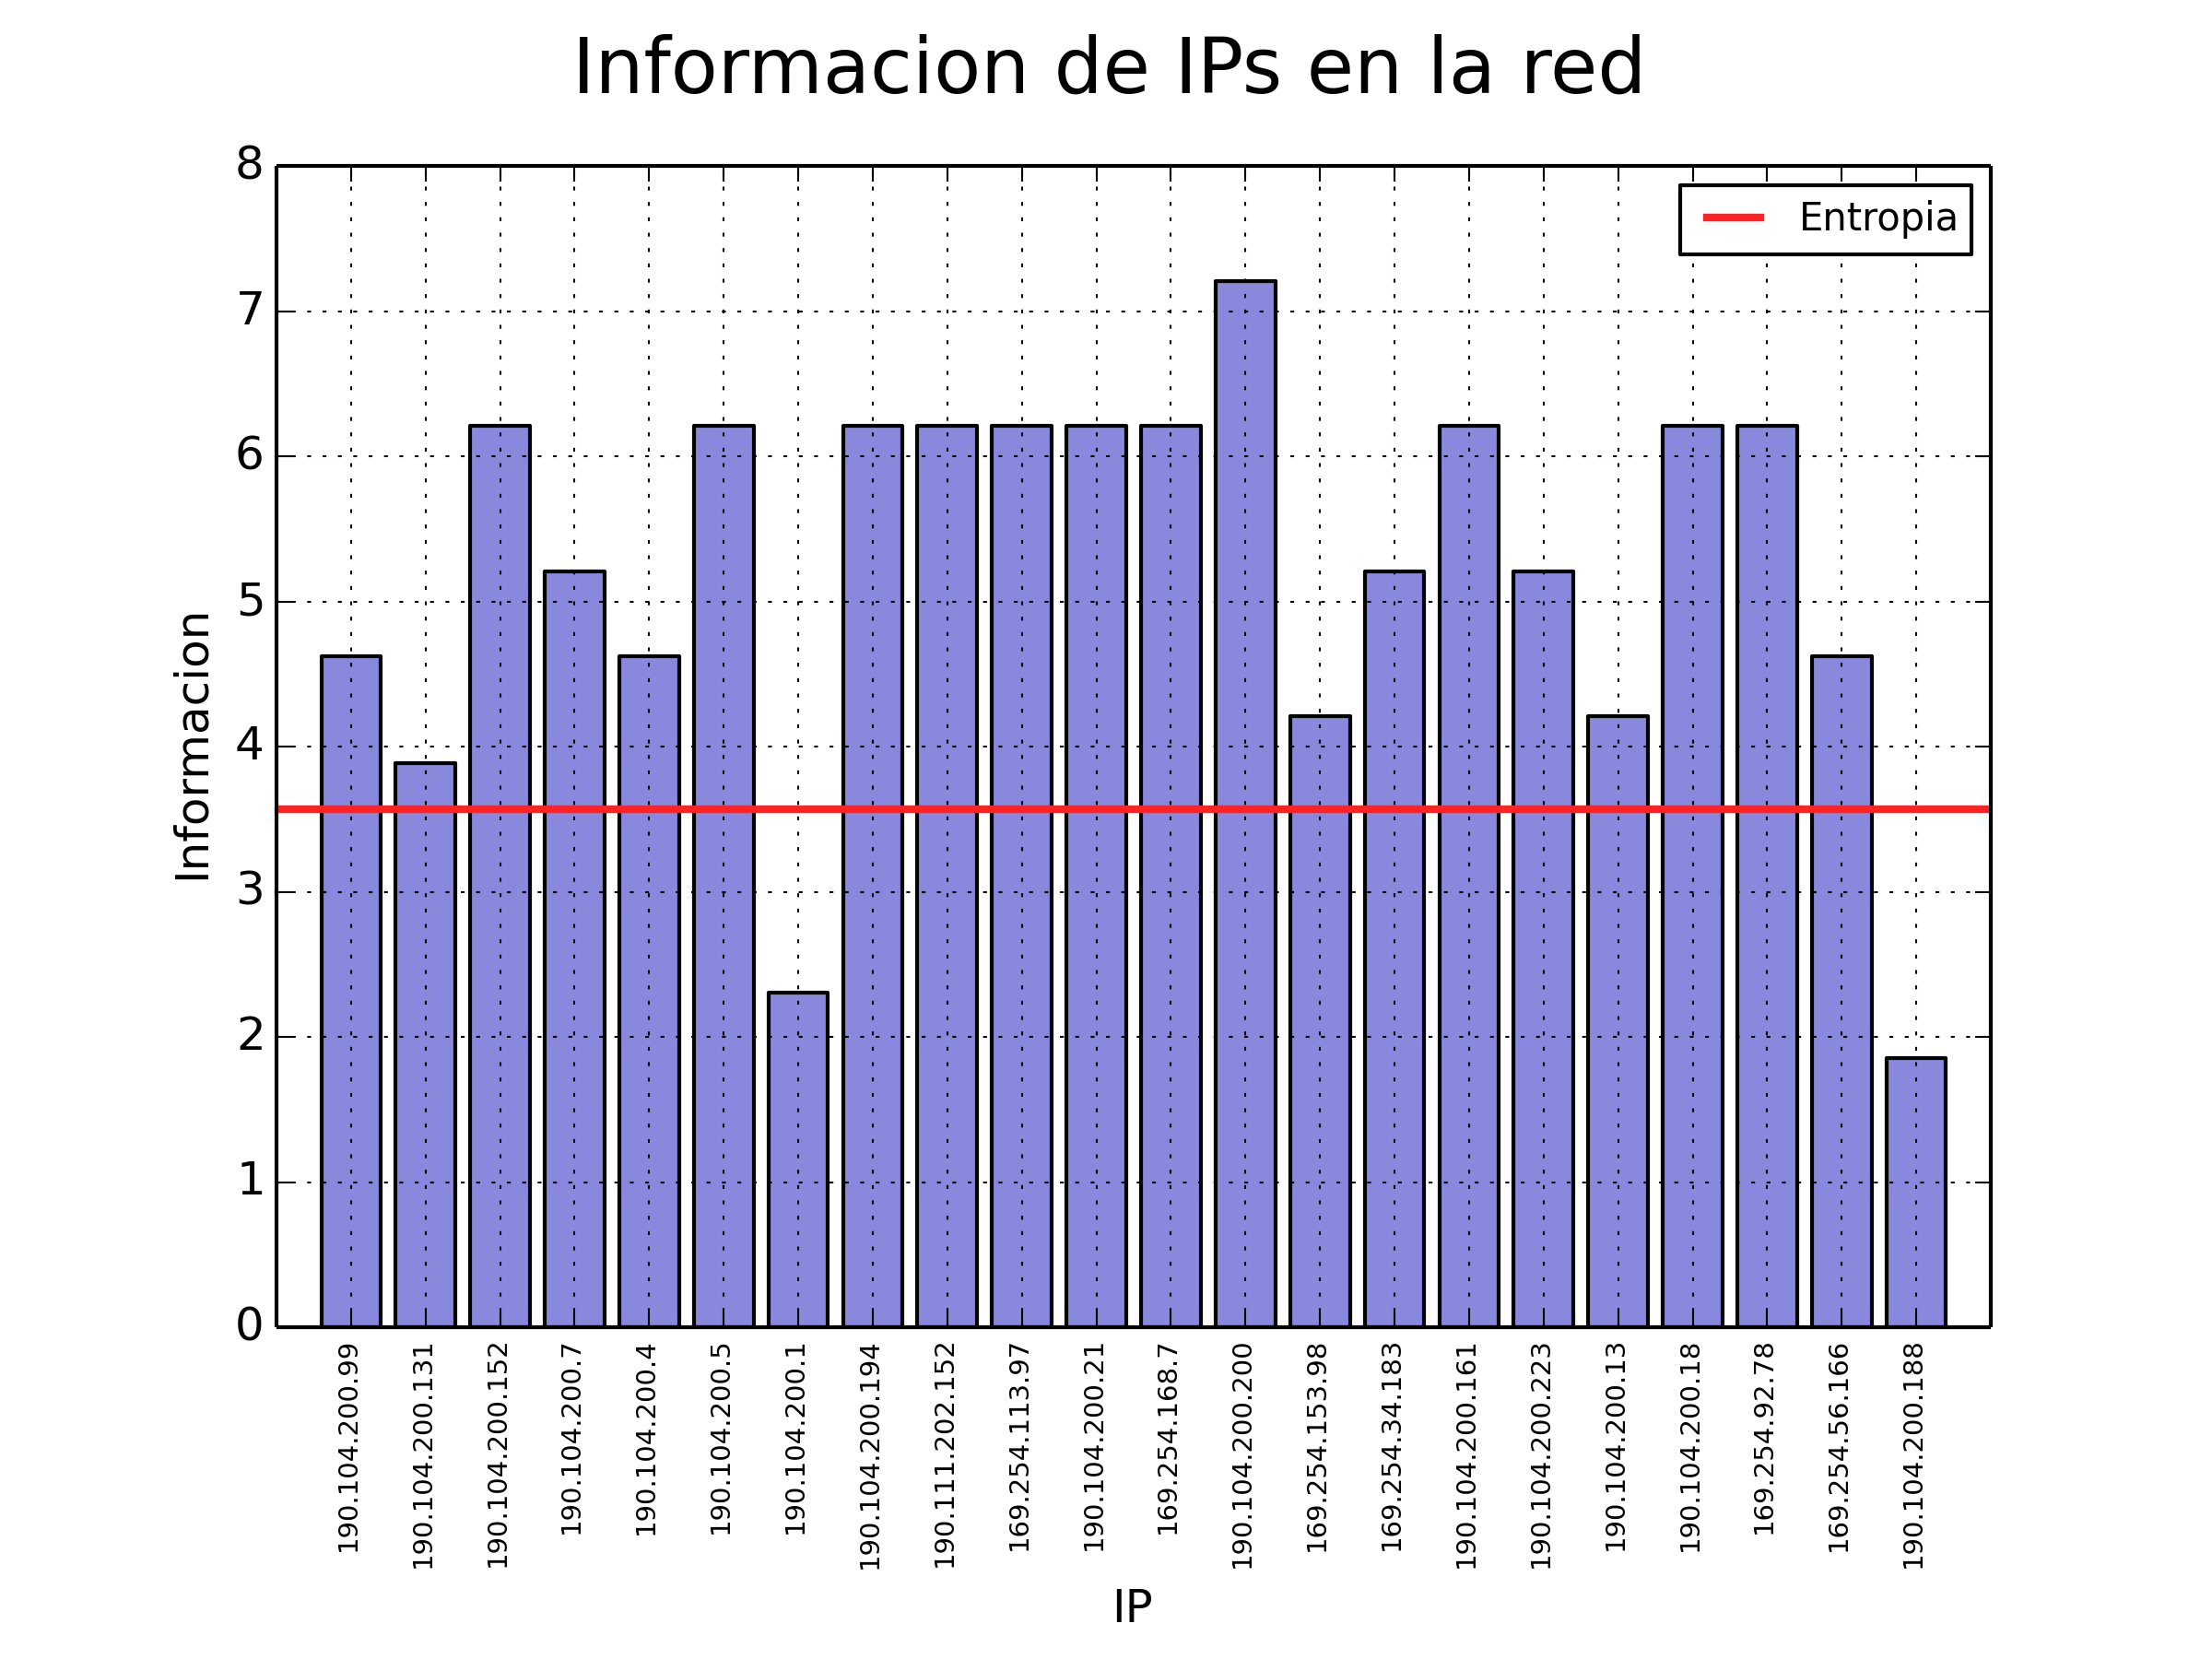
\includegraphics[width=0.7\textwidth]{graficos/shopping_information_bars_arp.png}
  \caption{}
  \label{fig:shopping_information_bars_arp}
\end{figure}

\FloatBarrier

Como podemos observar, hay dos nodos que presentan una cantidad de información que se encuentra por debajo de la entropía. Basándonos en los experimentos analizados anteriormente, inferimos que alguno de estos dos nodos posiblemente sea el router.
\\\\
Vemos el gráfico de la cantidad de información de cada protocolo en comparación con la entropía.

\FloatBarrier

\begin{figure}[ht!]
  \centering
   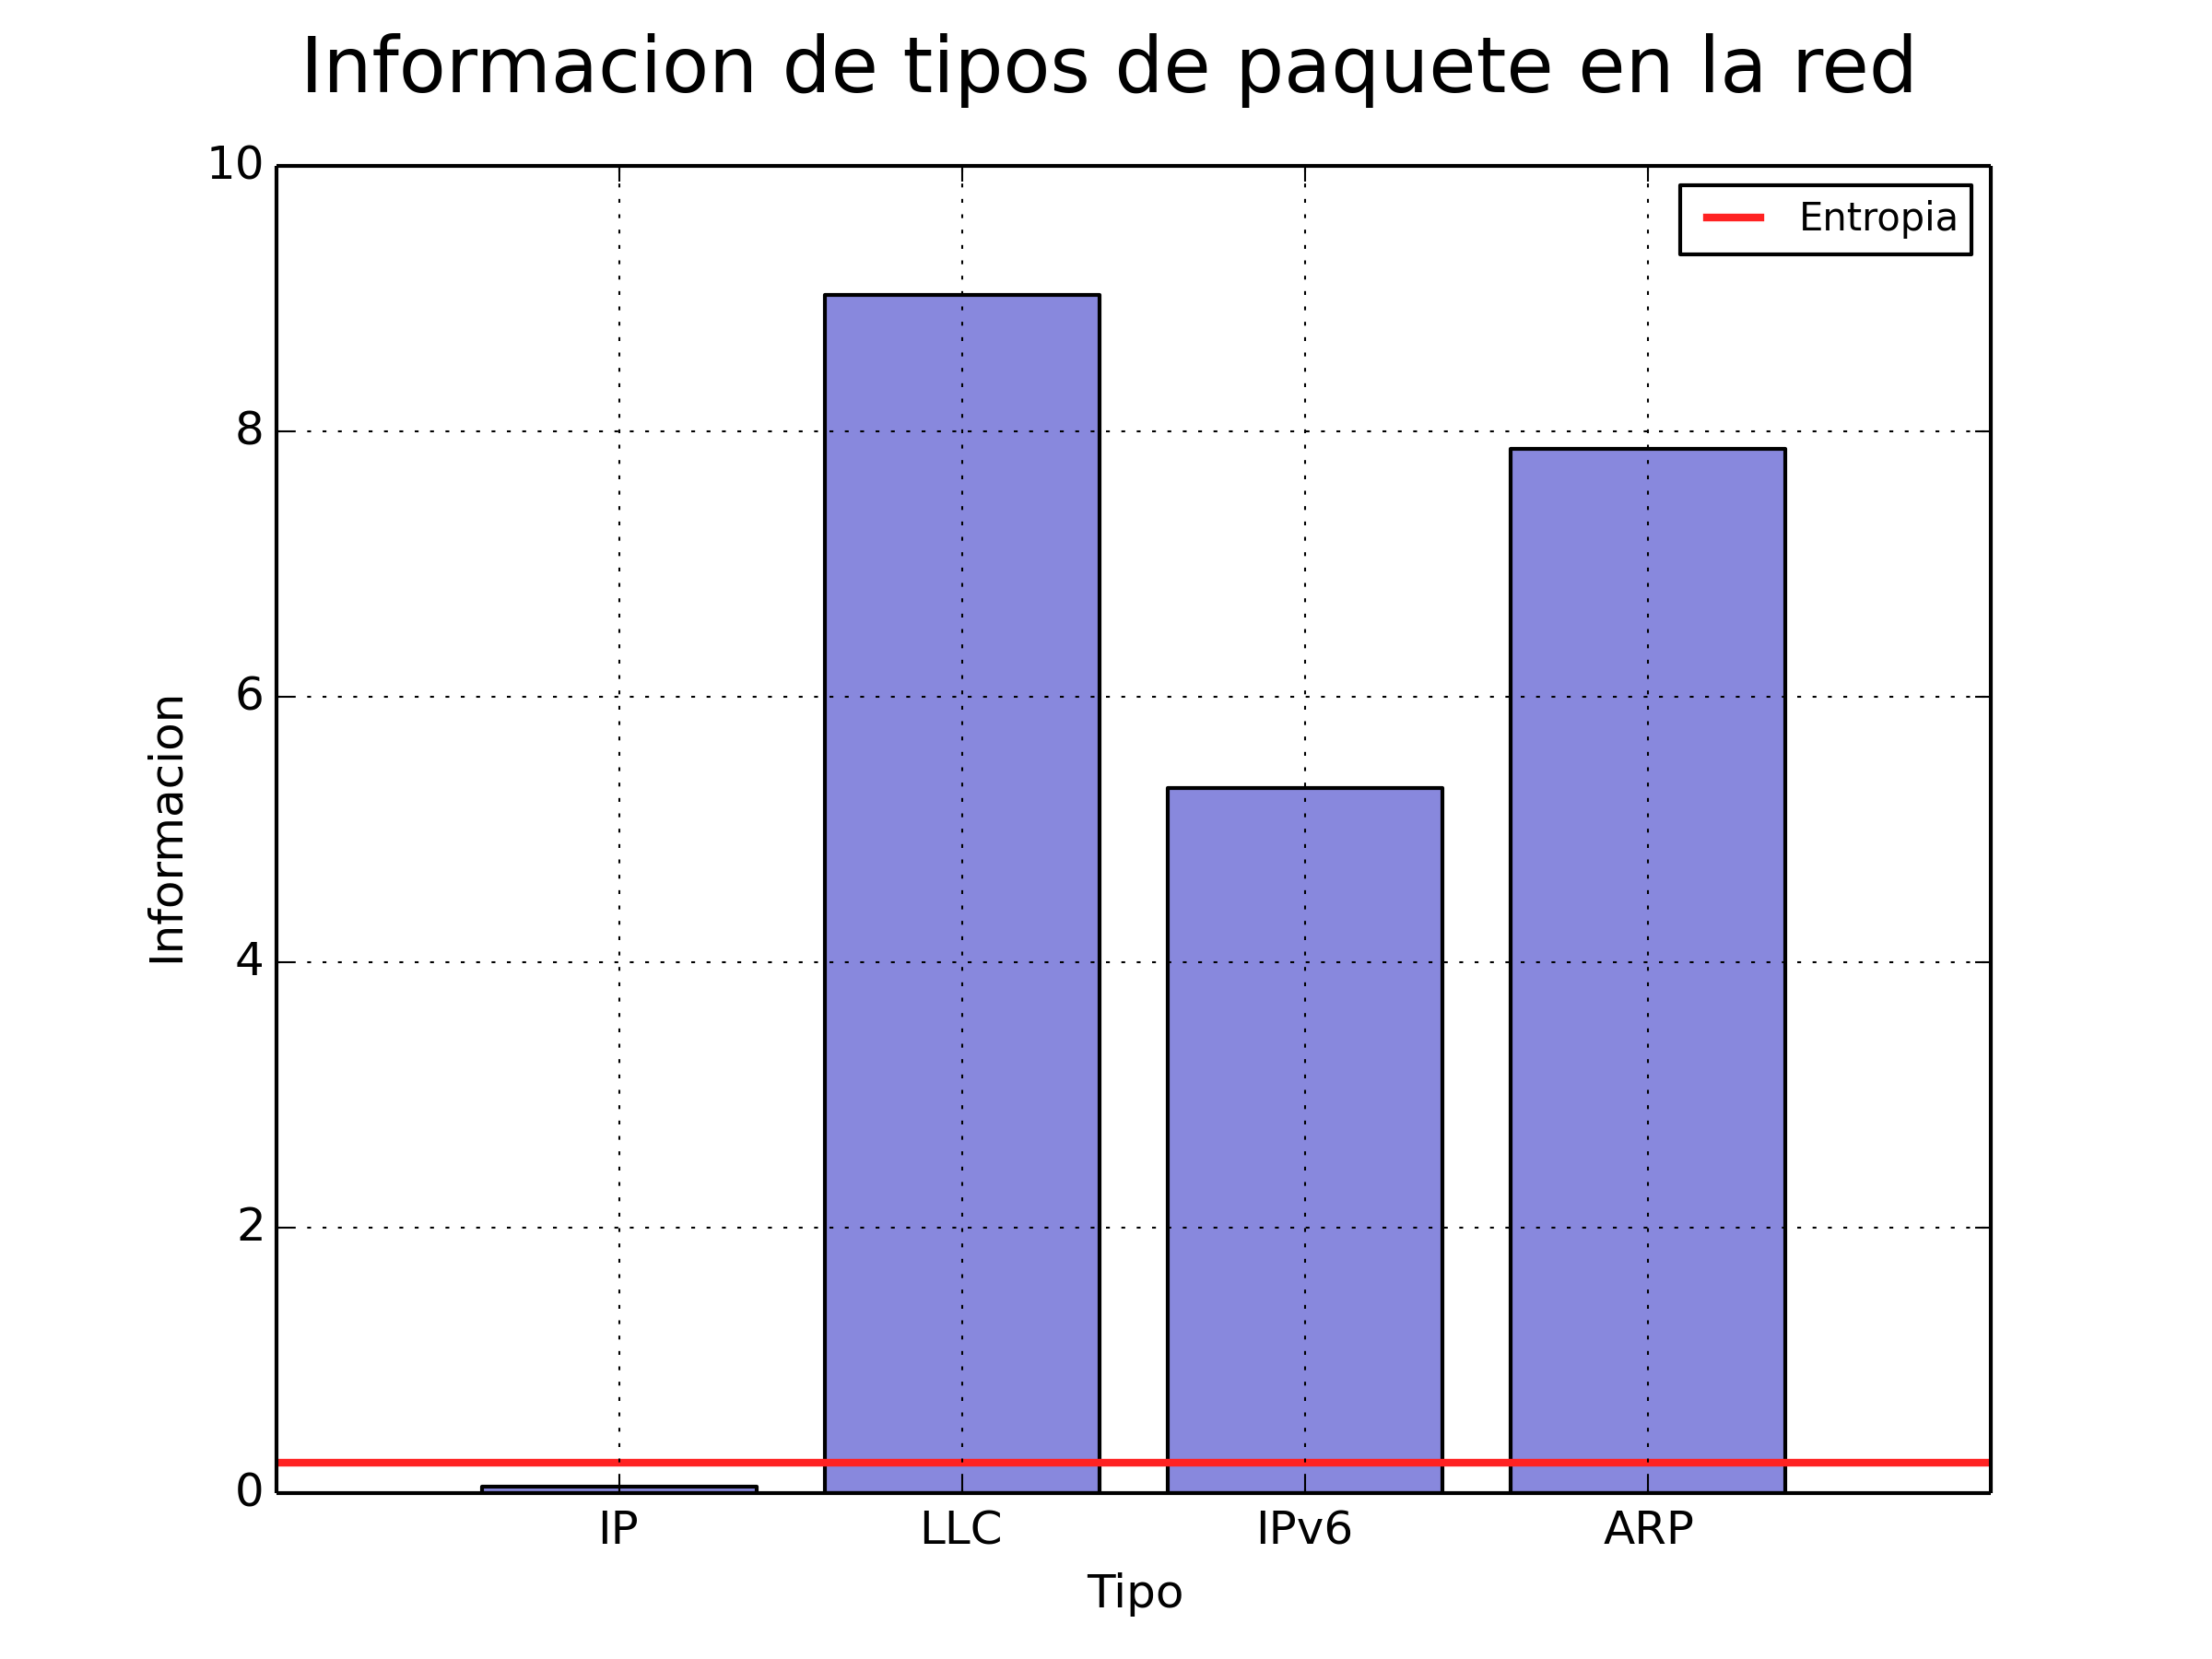
\includegraphics[width=0.7\textwidth]{graficos/shopping_information_bars_type.png}
  \caption{}
  \label{fig:shopping_information_bars_type}
\end{figure}

\FloatBarrier

En este caso los resultados son similares a los obtenidos en los experimentos anteriores. Donde el protocolo IP presenta una cantidad de información por debajo del valor de la entropía. El resto de los protocolos, LLC, IPv6 y ARP, aparecieron con menor frecuencia, aportando mayor cantidad de información.
%\pagebreak
%\section{Conclusiones}
En estos experimentos pudimos apreciar una aplicación concreta de la teoría de la información que nos permitió modelar y analizar diferentes fuentes de información.
\\\\
En la primera parte del trabajo práctico, al buscar protocolos distinguidos se descubrió que, en general, el protocolo más frecuente es el IPv4, lo cual es razonable. Además se notó que en algunas redes el protocolo IPv6, también, es bastante frecuente y que el protocolo ARP siempre se encontró presente en ellas. Esto último es previsible, por el funcionamiento de las redes IP en LAN.
\\\\
En el análisis de protocolos pudimos encontrar muchas similitudes entre las distintas redes. En general la entropía de esta fuente presentó un valor bajo y además el protocolo IPv4, que es el que mayor tráfico presenta, aportó valores de información inferiores. Esto demuestra una fuente predecible en la que se espera que la mayoría de los paquetes pertenezcan al protocolo IPv4.
\\\\
En la segunda parte del trabajo se investigó la existencia de nodos distinguidos (o símbolos distinguidos en el contexto de la fuente $S_1$).
\\\\
Se pudo observar que en las redes analizadas el router fue uno de los nodos distinguidos.
\\\\
También se observó que para las fuentes que modelan los diferentes nodos de la red, el valor de la entropía fue más elevado que la entropía de las fuentes que modelan los tipos de protocolos. Esto nos parece razonable debido a la impredecibilidad de la incidencia de los nodos en la red en comparación con la de los diferentes tipos de protocolos.


%\pagebreak



%\newpage
%\begin{thebibliography}{9}
 %\end{thebibliography}


\end{document}

